\chapter{Hands on Python \& OpenCV}
\label{sec:chap6}
Magnetic Resonance Imaging (MRI) helps the healthcare field detect very minor abnormal growth in any part of the human being. While deep neural networks (NNs) and machine learning techniques have good achievement in 2D image segmentation, but it’s a challenging task for NNs to segment critical organs from 3D medical MR images. Segmentation relating to tumor detection includes several processing techniques categorized into Pre-Processing, Segmentation, Optimization, and Feature Extraction.

\section{Introduction to OpenCV}

\subsection{Installing OpenCV for Python}

\subsubsection{Windows}

In order to get OpenCV-Python up and running, we need to perform the following steps:

\begin{enumerate}
	\item \textbf{Install Python}:Make sure you have Python 3.8.x installed on your machine. If you don't have it, you can install it from \url{https://www.python.org/downloads/windows/}
	
	\item \textbf{Install NumPy}: NumPy is a great package to do numerical computing in Python. It is very powerful and has a wide variety of functions. OpenCV-Python plays nicely with NumPy, and we will be using this package a lot, during the course of this book. You can install the latest version from \url{http://sourceforge.net/projects/numpy/files/NumPy/}. We need to install all these packages in their default locations. Once we install Python and NumPy, we need to ensure that they're working fine. Open up the Python shell and type the following:
	
	\vspace{0.5cm}
	\colorbox{lgray}{\\\textbf{$>>>$ import numpy as np}}
	\vspace{0.5cm}
	
	If the installation has gone well, this shouldn't throw any error
	
	\item \textbf{Install Matplotlib}: Matplotlib is a comprehensive library for creating static, animated, and interactive visualizations in Python. We use pip package to install this library. Type the folloing script in your command prompt. 
	
	\vspace{0.5cm}
	\colorbox{lgray}{\\\textbf{pip install matplotlib}}
	\vspace{0.5cm}
	
	\item \textbf{Install OpenCV}:download the latest OpenCV version from \url{http://opencv.org/downloads.html}. Once you finish downloading it, double-click to install it. You're all set! Let's make sure that OpenCV is working. Open up the Python shell and type the following:
	
	\vspace{0.5cm}
	\colorbox{lgray}{\\\textbf{$>>>$ import cv2}}
	\vspace{0.5cm}
\end{enumerate}

\subsubsection{Linux (for Ubuntu)}
Let’s go ahead and build OpenCV with Python support. The commands below will install all packages necessary to run OpenCV.

\vspace{0.5cm}
\colorbox{lgray}{\\\textbf{\$ sudo apt update}}

\colorbox{lgray}{\\\textbf{\$ sudo apt install python3-opencv}}
\vspace{0.5cm}

To verify the installation, import the cv2 module and print the OpenCV version:

\vspace{0.5cm}
\colorbox{lgray}{\\\textbf{$>>>$ import cv2}}

\colorbox{lgray}{\\\textbf{$>>>$ print (cv2.\_\_version\_\_)}}
\vspace{0.5cm}

\subsection{Reading, Displaying, and Saving images}
Let's see how we can load an image in OpenCV-Python. Create a new jupyter notebook named \textbf{program 1}.  Create a folder named \textbf{images} in the current folder, and make sure that you have at least one	image with .jpg format in that folder. Once you do that, add the following lines of code to one of the Python cells. If you run the preceding program, you will see an image being displayed in a new window.

\vspace{0.2cm}

\begin{tcolorbox}[breakable, size=fbox, boxrule=1pt, pad at break*=1mm,colback=cellbackground, colframe=cellborder]
	\prompt{In}{incolor}{ }{\boxspacing}
	\begin{Verbatim}[commandchars=\\\{\}]
\PY{k+kn}{import} \PY{n+nn}{cv2}
	\end{Verbatim}
\end{tcolorbox}

\begin{tcolorbox}[breakable, size=fbox, boxrule=1pt, pad at break*=1mm,colback=cellbackground, colframe=cellborder]
	\prompt{In}{incolor}{ }{\boxspacing}
	\begin{Verbatim}[commandchars=\\\{\}]
\PY{n}{img} \PY{o}{=} \PY{n}{cv2}\PY{o}{.}\PY{n}{imread}\PY{p}{(}\PY{l+s+s1}{\PYZsq{}}\PY{l+s+s1}{images/Sample1.jpg}\PY{l+s+s1}{\PYZsq{}}\PY{p}{)}
\PY{n}{cv2}\PY{o}{.}\PY{n}{imshow}\PY{p}{(}\PY{l+s+s1}{\PYZsq{}}\PY{l+s+s1}{Sample 1}\PY{l+s+s1}{\PYZsq{}}\PY{p}{,}\PY{n}{img}\PY{p}{)}
\PY{n}{cv2}\PY{o}{.}\PY{n}{waitKey}\PY{p}{(}\PY{p}{)}
	\end{Verbatim}
\end{tcolorbox}

\begin{figure}[htbp]
	\centering 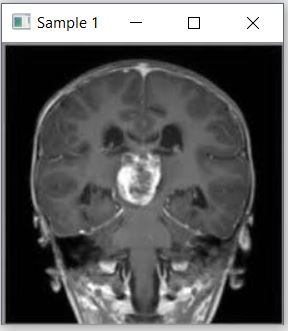
\includegraphics[width=0.45\columnwidth]{./figures/p1.jpg}
\end{figure}

Let's understand the previous piece of code, line by line. In the first line, we are importing the OpenCV 	library. We need this for all the functions we will be using in the code. In the second line, we are reading the image 	and storing it in a variable. OpenCV uses NumPy data structures to store the images. In the next line, we display the 	image in a new window. The first argument in \textbf{cv2.imshow} is the name of the window. The second argument is the 	image you want to display.

The function, \textbf{cv2.waitKey()}, is used in OpenCV for keyboard binding. It takes a number as an argument, and 	that number indicates the time in milliseconds. Basically, we use this function to wait for a specified duration, until we 	encounter a keyboard event. The program stops at this point, and waits for you to press any key to continue. If we 	don't pass any argument or if we pass 0 as the argument, this function will wait for a keyboard event indefinitely.

\subsection{Loading and Saving images}
OpenCV provides multiple ways of loading an image. Let's say we want to load a color image in grayscale mode. We can do that using the following piece of code:

\vspace{0.5cm}

\begin{tcolorbox}[breakable, size=fbox, boxrule=1pt, pad at break*=1mm,colback=cellbackground, colframe=cellborder]
	\prompt{In}{incolor}{ }{\boxspacing}
	\begin{Verbatim}[commandchars=\\\{\}]
\PY{k+kn}{import} \PY{n+nn}{cv2}
	\end{Verbatim}
\end{tcolorbox}

\begin{tcolorbox}[breakable, size=fbox, boxrule=1pt, pad at break*=1mm,colback=cellbackground, colframe=cellborder]
	\prompt{In}{incolor}{ }{\boxspacing}
	\begin{Verbatim}[commandchars=\\\{\}]
\PY{n}{normal\PYZus{}img} \PY{o}{=} \PY{n}{cv2}\PY{o}{.}\PY{n}{imread}\PY{p}{(}\PY{l+s+s1}{\PYZsq{}}\PY{l+s+s1}{images/Sample2.jpg}\PY{l+s+s1}{\PYZsq{}}\PY{p}{)}
\PY{n}{gray\PYZus{}img} \PY{o}{=} \PY{n}{cv2}\PY{o}{.}\PY{n}{imread}\PY{p}{(}\PY{l+s+s1}{\PYZsq{}}\PY{l+s+s1}{images/Sample2.jpg}\PY{l+s+s1}{\PYZsq{}}\PY{p}{,}\PY{n}{cv2}\PY{o}{.}\PY{n}{IMREAD\PYZus{}GRAYSCALE}\PY{p}{)}
\PY{n}{cv2}\PY{o}{.}\PY{n}{imshow}\PY{p}{(}\PY{l+s+s1}{\PYZsq{}}\PY{l+s+s1}{Normal image}\PY{l+s+s1}{\PYZsq{}}\PY{p}{,}\PY{n}{normal\PYZus{}img}\PY{p}{)}
\PY{n}{cv2}\PY{o}{.}\PY{n}{imshow}\PY{p}{(}\PY{l+s+s1}{\PYZsq{}}\PY{l+s+s1}{Gray Scale image}\PY{l+s+s1}{\PYZsq{}}\PY{p}{,}\PY{n}{gray\PYZus{}img}\PY{p}{)}
\PY{n}{cv2}\PY{o}{.}\PY{n}{waitKey}\PY{p}{(}\PY{p}{)}
	\end{Verbatim}
\end{tcolorbox}

\begin{figure}[htbp]
	\centerline{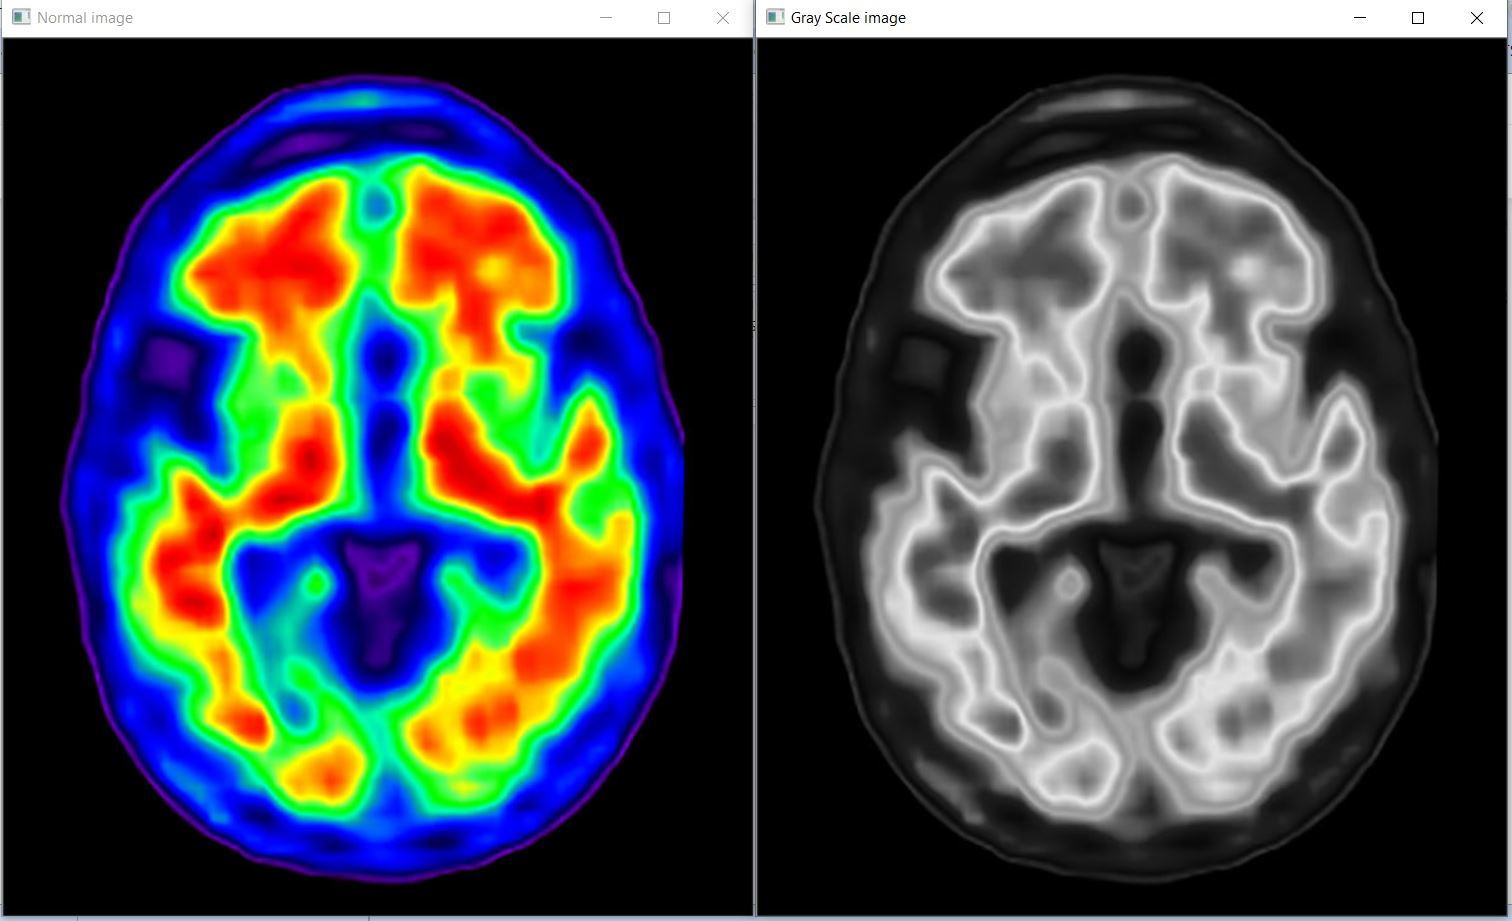
\includegraphics[width=0.8\columnwidth]{figures/p2.jpg}}
\end{figure}

Here, we are using the flag \textbf{cv2.IMREAD\_GRAYSCALE} to load the image in grayscale mode. You can see that from the 	image being displayed in the new window. We can save this image into a file as well:

\vspace{0.5cm}

\begin{tcolorbox}[breakable, size=fbox, boxrule=1pt, pad at break*=1mm,colback=cellbackground, colframe=cellborder]
	\prompt{In}{incolor}{ }{\boxspacing}
	\begin{Verbatim}[commandchars=\\\{\}]
\PY{n}{cv2}\PY{o}{.}\PY{n}{imwrite}\PY{p}{(}\PY{l+s+s1}{\PYZsq{}}\PY{l+s+s1}{images/output.jpg}\PY{l+s+s1}{\PYZsq{}}\PY{p}{,}\PY{n}{gray\PYZus{}img}\PY{p}{)}
	\end{Verbatim}
\end{tcolorbox}

This will save the grayscale image into an output file named \textbf{output.jpg}.

\subsection{Image color spaces}
In computer vision and image processing, color space refers to a specific way of organizing colors. A color space is actually a combination of two things: a color model and a mapping function. The reason we want color models is because it helps us in representing pixel values using tuples. The mapping function maps the color model to the set of all possible colors that can be represented.

There are many different color spaces that are useful. Some of the more popular color spaces are RGB, YUV, 	HSV, Lab, and so on. Different color spaces provide different advantages. We just need to pick the color space that's 	right for the given problem. Let's take a couple of color spaces and see what information they provide:

\begin{itemize}
	\item \textbf{RGB}: It's probably the most popular color space. It stands for Red, Green, and Blue. In this color space, each 	color is represented as a weighted combination of red, green, and blue. So every pixel value is represented as a tuple 	of three numbers corresponding to red, green, and blue. Each value ranges between 0 and 255.
	
	\item \textbf{YUV}: Even though RGB is good for many purposes, it tends to be very limited for many real life applications. 	People started thinking about different methods to separate the intensity information from the color information. 	Hence, they came up with the YUV color space. Y refers to the luminance or intensity, and U/V channels represent 	color information. This works well in many applications because the human visual system perceives intensity 	information very differently from color information.
	
	\item \textbf{HSV}: : As it turned out, even YUV was still not good enough for some of the applications. So people started 	thinking about how humans perceive color and they came up with the HSV color space. HSV stands for Hue, Saturation, 	and Value. This is a cylindrical system where we separate three of the most primary properties of colors and represent 	them using different channels. This is closely related to how the human visual system understands color. This gives us a lot of flexibility as to how we can handle images.
\end{itemize}

\subsection{Converting between color spaces}

Considering all the color spaces, there are around 190 conversion options available in OpenCV. If you want to see a list of first 30 available flags, type the following codes in your Jupyter notebook:

\begin{tcolorbox}[breakable, size=fbox, boxrule=1pt, pad at break*=1mm,colback=cellbackground, colframe=cellborder]
	\prompt{In}{incolor}{ }{\boxspacing}
	\begin{Verbatim}[commandchars=\\\{\}]
\PY{k+kn}{import} \PY{n+nn}{cv2}
	\end{Verbatim}
\end{tcolorbox}

\begin{tcolorbox}[breakable, size=fbox, boxrule=1pt, pad at break*=1mm,colback=cellbackground, colframe=cellborder]
\prompt{In}{incolor}{ }{\boxspacing}
\begin{Verbatim}[commandchars=\\\{\}]
\PY{n}{i} \PY{o}{=} \PY{l+m+mi}{0}
\PY{k}{for} \PY{n}{x} \PY{o+ow}{in} \PY{n+nb}{dir}\PY{p}{(}\PY{n}{cv2}\PY{p}{)}\PY{p}{:}
    \PY{k}{if}\PY{p}{(}\PY{n}{x}\PY{o}{.}\PY{n}{startswith}\PY{p}{(}\PY{l+s+s1}{\PYZsq{}}\PY{l+s+s1}{COLOR\PYZus{}}\PY{l+s+s1}{\PYZsq{}}\PY{p}{)} \PY{o+ow}{and} \PY{n}{i}\PY{o}{\PYZlt{}}\PY{l+m+mi}{50}\PY{p}{)}\PY{p}{:}
        \PY{n+nb}{print}\PY{p}{(}\PY{n}{x}\PY{p}{,}\PY{n}{end}\PY{o}{=}\PY{l+s+s1}{\PYZsq{}}\PY{l+s+s1}{ , }\PY{l+s+s1}{\PYZsq{}}\PY{p}{)}
        \PY{n}{i} \PY{o}{+}\PY{o}{=} \PY{l+m+mi}{1}
\end{Verbatim}
\end{tcolorbox}

\begin{Verbatim}[commandchars=\\\{\}]
COLOR\_BAYER\_BG2BGR , COLOR\_BAYER\_BG2BGRA , COLOR\_BAYER\_BG2BGR\_EA ,
COLOR\_BAYER\_BG2BGR\_VNG , COLOR\_BAYER\_BG2GRAY , COLOR\_BAYER\_BG2RGB ,
COLOR\_BAYER\_BG2RGBA , COLOR\_BAYER\_BG2RGB\_EA , COLOR\_BAYER\_BG2RGB\_VNG ,
COLOR\_BAYER\_GB2BGR , COLOR\_BAYER\_GB2BGRA , COLOR\_BAYER\_GB2BGR\_EA ,
COLOR\_BAYER\_GB2BGR\_VNG , COLOR\_BAYER\_GB2GRAY , COLOR\_BAYER\_GB2RGB ,
COLOR\_BAYER\_GB2RGBA , COLOR\_BAYER\_GB2RGB\_EA , COLOR\_BAYER\_GB2RGB\_VNG ,
COLOR\_BAYER\_GR2BGR , COLOR\_BAYER\_GR2BGRA , COLOR\_BAYER\_GR2BGR\_EA ,
COLOR\_BAYER\_GR2BGR\_VNG , COLOR\_BAYER\_GR2GRAY , COLOR\_BAYER\_GR2RGB ,
COLOR\_BAYER\_GR2RGBA , COLOR\_BAYER\_GR2RGB\_EA , COLOR\_BAYER\_GR2RGB\_VNG ,
COLOR\_BAYER\_RG2BGR , COLOR\_BAYER\_RG2BGRA , COLOR\_BAYER\_RG2BGR\_EA ,
COLOR\_BAYER\_RG2BGR\_VNG , COLOR\_BAYER\_RG2GRAY , COLOR\_BAYER\_RG2RGB ,
COLOR\_BAYER\_RG2RGBA , COLOR\_BAYER\_RG2RGB\_EA , COLOR\_BAYER\_RG2RGB\_VNG ,
COLOR\_BGR2BGR555 , COLOR\_BGR2BGR565 , COLOR\_BGR2BGRA , COLOR\_BGR2GRAY ,
COLOR\_BGR2HLS , COLOR\_BGR2HLS\_FULL , COLOR\_BGR2HSV , COLOR\_BGR2HSV\_FULL ,
COLOR\_BGR2LAB , COLOR\_BGR2LUV , COLOR\_BGR2Lab , COLOR\_BGR2Luv ,
COLOR\_BGR2RGB , COLOR\_BGR2RGBA 
\end{Verbatim}

\vspace{0.5cm}

You will see a list of options available in OpenCV for converting from one color space to another. We can pretty 	much convert any color space into any other color space. 

\section{Geometric Transformations}

\subsection{Image Translation}
In this section, we will discuss about shifting an image. Let's say we want to move the image within our frame of reference. In computer vision terminology, this is referred to as translation. Let's go ahead and see how we can do 	that:

\vspace{0.5cm}

\begin{tcolorbox}[breakable, size=fbox, boxrule=1pt, pad at break*=1mm,colback=cellbackground, colframe=cellborder]
	\prompt{In}{incolor}{ }{\boxspacing}
	\begin{Verbatim}[commandchars=\\\{\}]
\PY{k+kn}{import} \PY{n+nn}{cv2}
\PY{k+kn}{import} \PY{n+nn}{numpy} \PY{k}{as} \PY{n+nn}{np}
\PY{k+kn}{import} \PY{n+nn}{matplotlib}\PY{n+nn}{.}\PY{n+nn}{pyplot} \PY{k}{as} \PY{n+nn}{plt}
	\end{Verbatim}
\end{tcolorbox}

\begin{tcolorbox}[breakable, size=fbox, boxrule=1pt, pad at break*=1mm,colback=cellbackground, colframe=cellborder]
	\prompt{In}{incolor}{ }{\boxspacing}
	\begin{Verbatim}[commandchars=\\\{\}]
\PY{n}{img} \PY{o}{=} \PY{n}{cv2}\PY{o}{.}\PY{n}{imread}\PY{p}{(}\PY{l+s+s1}{\PYZsq{}}\PY{l+s+s1}{images/Sample3.png}\PY{l+s+s1}{\PYZsq{}}\PY{p}{)}
\PY{n}{num\PYZus{}rows}\PY{p}{,} \PY{n}{num\PYZus{}cols} \PY{o}{=} \PY{n}{img}\PY{o}{.}\PY{n}{shape}\PY{p}{[}\PY{p}{:}\PY{l+m+mi}{2}\PY{p}{]}
		
\PY{n+nb}{print}\PY{p}{(}\PY{l+s+s1}{\PYZsq{}}\PY{l+s+s1}{rows:}\PY{l+s+si}{\PYZob{}0\PYZcb{}}\PY{l+s+s1}{\PYZsq{}}\PY{o}{.}\PY{n}{format}\PY{p}{(}\PY{n}{num\PYZus{}rows}\PY{p}{)}\PY{p}{)}
\PY{n+nb}{print}\PY{p}{(}\PY{l+s+s1}{\PYZsq{}}\PY{l+s+s1}{columns:}\PY{l+s+si}{\PYZob{}0\PYZcb{}}\PY{l+s+s1}{\PYZsq{}}\PY{o}{.}\PY{n}{format}\PY{p}{(}\PY{n}{num\PYZus{}cols}\PY{p}{)}\PY{p}{)}
	\end{Verbatim}
\end{tcolorbox}

\begin{Verbatim}[commandchars=\\\{\}]
rows:410
columns:410
\end{Verbatim}

\begin{tcolorbox}[breakable, size=fbox, boxrule=1pt, pad at break*=1mm,colback=cellbackground, colframe=cellborder]
	\prompt{In}{incolor}{ }{\boxspacing}
	\begin{Verbatim}[commandchars=\\\{\}]
\PY{n}{translation\PYZus{}matrix} \PY{o}{=} \PY{n}{np}\PY{o}{.}\PY{n}{float32}\PY{p}{(}\PY{p}{[} \PY{p}{[}\PY{l+m+mi}{1}\PY{p}{,}\PY{l+m+mi}{0}\PY{p}{,}\PY{l+m+mi}{70}\PY{p}{]}\PY{p}{,} \PY{p}{[}\PY{l+m+mi}{0}\PY{p}{,}\PY{l+m+mi}{1}\PY{p}{,}\PY{l+m+mi}{110}\PY{p}{]} \PY{p}{]}\PY{p}{)}
\PY{n}{img\PYZus{}translation} \PY{o}{=} \PY{n}{cv2}\PY{o}{.}\PY{n}{warpAffine}\PY{p}{(}\PY{n}{img}\PY{p}{,} \PY{n}{translation\PYZus{}matrix}\PY{p}{,} \PY{p}{(}\PY{n}{num\PYZus{}cols}\PY{p}{,}
\PY{n}{num\PYZus{}rows}\PY{p}{)}\PY{p}{)}
	\end{Verbatim}
\end{tcolorbox}

\begin{tcolorbox}[breakable, size=fbox, boxrule=1pt, pad at break*=1mm,colback=cellbackground, colframe=cellborder]
	\prompt{In}{incolor}{ }{\boxspacing}
	\begin{Verbatim}[commandchars=\\\{\}]
\PY{n}{fig}\PY{p}{,} \PY{n}{axs} \PY{o}{=} \PY{n}{plt}\PY{o}{.}\PY{n}{subplots}\PY{p}{(}\PY{l+m+mi}{1}\PY{p}{,}\PY{l+m+mi}{2}\PY{p}{,}\PY{n}{figsize}\PY{o}{=}\PY{p}{(}\PY{l+m+mi}{10}\PY{p}{,}\PY{l+m+mi}{5}\PY{p}{)}\PY{p}{)}
\PY{n}{axs}\PY{p}{[}\PY{l+m+mi}{0}\PY{p}{]}\PY{o}{.}\PY{n}{imshow}\PY{p}{(}\PY{n}{img}\PY{p}{)}
\PY{n}{axs}\PY{p}{[}\PY{l+m+mi}{1}\PY{p}{]}\PY{o}{.}\PY{n}{imshow}\PY{p}{(}\PY{n}{img\PYZus{}translation}\PY{p}{)}
	\end{Verbatim}
\end{tcolorbox}

\begin{tcolorbox}[breakable, size=fbox, boxrule=.5pt, pad at break*=1mm, opacityfill=0]
	\prompt{Out}{outcolor}{ }{\boxspacing}
	\begin{Verbatim}[commandchars=\\\{\}]
<matplotlib.image.AxesImage at 0x273d77da430>
	\end{Verbatim}
\end{tcolorbox}

\begin{center}
	\adjustimage{max size={0.9\linewidth}{0.9\paperheight}}{figures/p5.png}
\end{center}
{ \hspace*{\fill} \\}

To understand the preceding code, we need to understand how warping works. Translation basically means that we are shifting the image by adding/subtracting the X and Y coordinates. In order to do this, we need to create a transformation matrix, as shown as follows:

\begin{center}
\[
\textit{T} =  
\begin{bmatrix}
	1 & 0 & t_{x} \\
	0 & 1 & t_{y}
\end{bmatrix}
\]
\end{center}

Here, the $t_x$ and $t_y$ values are the \textit{X} and \textit{Y} translation values, that is, the image will be moved by \textit{X} units towards 	the right, and by \textit{Y} units downwards. So once we create a matrix like this, we can use the function, warpAffine, to 	apply to our image. The third argument in \textbf{warpAffine} refers to the number of rows and columns in the resulting image. Since the number of rows and columns is the same as the original image, the resultant image is going to get cropped. The reason for this is because we didn't have enough space in the output when we applied the translation matrix. To 	avoid cropping, we can pass a bigger row size and column size in the third argument.

\subsection{Image Rotation}
Now, we will see how to rotate a given image by a certain angle. We can do it using the following piece of code:

\vspace{0.5cm}

\begin{tcolorbox}[breakable, size=fbox, boxrule=1pt, pad at break*=1mm,colback=cellbackground, colframe=cellborder]
	\prompt{In}{incolor}{ }{\boxspacing}
	\begin{Verbatim}[commandchars=\\\{\}]
\PY{k+kn}{import} \PY{n+nn}{cv2}
\PY{k+kn}{import} \PY{n+nn}{numpy} \PY{k}{as} \PY{n+nn}{np}
\PY{k+kn}{import} \PY{n+nn}{matplotlib}\PY{n+nn}{.}\PY{n+nn}{pyplot} \PY{k}{as} \PY{n+nn}{plt}
	\end{Verbatim}
\end{tcolorbox}

\begin{tcolorbox}[breakable, size=fbox, boxrule=1pt, pad at break*=1mm,colback=cellbackground, colframe=cellborder]
	\prompt{In}{incolor}{ }{\boxspacing}
	\begin{Verbatim}[commandchars=\\\{\}]
\PY{n}{img} \PY{o}{=} \PY{n}{cv2}\PY{o}{.}\PY{n}{imread}\PY{p}{(}\PY{l+s+s1}{\PYZsq{}}\PY{l+s+s1}{images/Sample4.jpg}\PY{l+s+s1}{\PYZsq{}}\PY{p}{)}
\PY{n}{num\PYZus{}rows}\PY{p}{,} \PY{n}{num\PYZus{}cols} \PY{o}{=} \PY{n}{img}\PY{o}{.}\PY{n}{shape}\PY{p}{[}\PY{p}{:}\PY{l+m+mi}{2}\PY{p}{]}
		
\PY{n+nb}{print}\PY{p}{(}\PY{l+s+s1}{\PYZsq{}}\PY{l+s+s1}{Rows : }\PY{l+s+si}{\PYZob{}\PYZcb{}}\PY{l+s+s1}{\PYZsq{}}\PY{o}{.}\PY{n}{format}\PY{p}{(}\PY{n}{num\PYZus{}rows}\PY{p}{)}\PY{p}{)}
\PY{n+nb}{print}\PY{p}{(}\PY{l+s+s1}{\PYZsq{}}\PY{l+s+s1}{Columns : }\PY{l+s+si}{\PYZob{}\PYZcb{}}\PY{l+s+s1}{\PYZsq{}}\PY{o}{.}\PY{n}{format}\PY{p}{(}\PY{n}{num\PYZus{}cols}\PY{p}{)}\PY{p}{)}
	\end{Verbatim}
\end{tcolorbox}

\begin{Verbatim}[commandchars=\\\{\}]
Rows : 350
Columns : 350
\end{Verbatim}

\begin{tcolorbox}[breakable, size=fbox, boxrule=1pt, pad at break*=1mm,colback=cellbackground, colframe=cellborder]
	\prompt{In}{incolor}{ }{\boxspacing}
	\begin{Verbatim}[commandchars=\\\{\}]
\PY{n}{rotation\PYZus{}matrix}\PY{o}{=}\PY{n}{cv2}\PY{o}{.}\PY{n}{getRotationMatrix2D}\PY{p}{(}\PY{p}{(}\PY{n}{num\PYZus{}cols}\PY{o}{/}\PY{l+m+mi}{2}\PY{p}{,} \PY{n}{num\PYZus{}rows}\PY{o}{/}\PY{l+m+mi}{2}\PY{p}{)}\PY{p}{,} \PY{l+m+mi}{30}\PY{p}{,} \PY{l+m+mi}{1}\PY{p}{)}
\PY{n}{img\PYZus{}rotation}\PY{o}{=}\PY{n}{cv2}\PY{o}{.}\PY{n}{warpAffine}\PY{p}{(}\PY{n}{img}\PY{p}{,}\PY{n}{rotation\PYZus{}matrix}\PY{p}{,}\PY{p}{(}\PY{n}{num\PYZus{}cols}\PY{p}{,}\PY{n}{num\PYZus{}rows}\PY{p}{)}\PY{p}{)}                                
	\end{Verbatim}
\end{tcolorbox}

\begin{tcolorbox}[breakable, size=fbox, boxrule=1pt, pad at break*=1mm,colback=cellbackground, colframe=cellborder]
	\prompt{In}{incolor}{ }{\boxspacing}
	\begin{Verbatim}[commandchars=\\\{\}]
\PY{n}{fig}\PY{p}{,} \PY{n}{axs} \PY{o}{=} \PY{n}{plt}\PY{o}{.}\PY{n}{subplots}\PY{p}{(}\PY{l+m+mi}{1}\PY{p}{,}\PY{l+m+mi}{2}\PY{p}{,}\PY{n}{figsize}\PY{o}{=}\PY{p}{(}\PY{l+m+mi}{10}\PY{p}{,}\PY{l+m+mi}{5}\PY{p}{)}\PY{p}{)}
		
\PY{n}{axs}\PY{p}{[}\PY{l+m+mi}{0}\PY{p}{]}\PY{o}{.}\PY{n}{imshow}\PY{p}{(}\PY{n}{img}\PY{p}{)}
\PY{n}{axs}\PY{p}{[}\PY{l+m+mi}{0}\PY{p}{]}\PY{o}{.}\PY{n}{set\PYZus{}title}\PY{p}{(}\PY{l+s+s1}{\PYZsq{}}\PY{l+s+s1}{Orginal Image}\PY{l+s+s1}{\PYZsq{}}\PY{p}{)}
		
\PY{n}{axs}\PY{p}{[}\PY{l+m+mi}{1}\PY{p}{]}\PY{o}{.}\PY{n}{imshow}\PY{p}{(}\PY{n}{img\PYZus{}rotation}\PY{p}{)}
\PY{n}{axs}\PY{p}{[}\PY{l+m+mi}{1}\PY{p}{]}\PY{o}{.}\PY{n}{set\PYZus{}title}\PY{p}{(}\PY{l+s+s1}{\PYZsq{}}\PY{l+s+s1}{Rotated Image}\PY{l+s+s1}{\PYZsq{}}\PY{p}{)}
	\end{Verbatim}
\end{tcolorbox}


\begin{tcolorbox}[breakable, size=fbox, boxrule=.5pt, pad at break*=1mm, opacityfill=0]
	\prompt{Out}{outcolor}{ }{\boxspacing}
	\begin{Verbatim}[commandchars=\\\{\}]
Text(0.5, 1.0, 'Rotated Image')
	\end{Verbatim}
\end{tcolorbox}

\begin{center}
	\adjustimage{max size={0.9\linewidth}{0.9\paperheight}}{figures/p6.png}
\end{center}
{ \hspace*{\fill} \\}

In order to understand this, let's see how we handle rotation mathematically. Rotation is also a form of transformation, and we can achieve it by using the following transformation matrix:

\begin{center}
	\[
	\textit{R} =  
	\begin{bmatrix}
		\cos\theta & -\sin\theta \\
		\sin\theta & \cos\theta
	\end{bmatrix}
	\]
\end{center}

Here, $\theta$ is the angle of rotation in the counterclockwise direction. OpenCV provides closer control over the creation of this matrix through the function, \textbf{getRotationMatrix2D}. We can specify the point around which the image would be rotated, the angle of rotation in degrees, and a scaling factor for the image. Once we have the transformation matrix, we can use the \textbf{warpAffine} function to apply this matrix to any image.

\subsection{Image Scaling}
In this section, we will discuss about resizing an image. This is one of the most common operations in computer 	vision. We can resize an image using a scaling factor, or we can resize it to a particular size. Let's see how to do that:

\vspace{0.5cm}

\begin{tcolorbox}[breakable, size=fbox, boxrule=1pt, pad at break*=1mm,colback=cellbackground, colframe=cellborder]
	\prompt{In}{incolor}{ }{\boxspacing}
	\begin{Verbatim}[commandchars=\\\{\}]
\PY{k+kn}{import} \PY{n+nn}{cv2}
\PY{k+kn}{import} \PY{n+nn}{matplotlib}\PY{n+nn}{.}\PY{n+nn}{pyplot} \PY{k}{as} \PY{n+nn}{plt}
	\end{Verbatim}
\end{tcolorbox}

\begin{tcolorbox}[breakable, size=fbox, boxrule=1pt, pad at break*=1mm,colback=cellbackground, colframe=cellborder]
	\prompt{In}{incolor}{ }{\boxspacing}
	\begin{Verbatim}[commandchars=\\\{\}]
\PY{n}{img} \PY{o}{=} \PY{n}{cv2}\PY{o}{.}\PY{n}{imread}\PY{p}{(}\PY{l+s+s1}{\PYZsq{}}\PY{l+s+s1}{images/Sample5.jpg}\PY{l+s+s1}{\PYZsq{}}\PY{p}{)}
\PY{n+nb}{print}\PY{p}{(}\PY{l+s+s1}{\PYZsq{}}\PY{l+s+s1}{Orginal image: }\PY{l+s+si}{\PYZob{}\PYZcb{}}\PY{l+s+s1}{\PYZsq{}}\PY{o}{.}\PY{n}{format}\PY{p}{(}\PY{n}{img}\PY{o}{.}\PY{n}{shape}\PY{p}{)}\PY{p}{)}


\PY{n}{img\PYZus{}scaled\PYZus{}Linear} \PY{o}{=} \PY{n}{cv2}\PY{o}{.}\PY{n}{resize}\PY{p}{(}\PY{n}{img}\PY{p}{,}\PY{k+kc}{None}\PY{p}{,}\PY{n}{fx}\PY{o}{=}\PY{l+m+mf}{1.5}\PY{p}{,} \PY{n}{fy}\PY{o}{=}\PY{l+m+mf}{1.5}\PY{p}{,} \PY{n}{interpolation} \PY{o}{=}
\PY{n}{cv2}\PY{o}{.}\PY{n}{INTER\PYZus{}LINEAR}\PY{p}{)}
\PY{n+nb}{print}\PY{p}{(}\PY{l+s+s1}{\PYZsq{}}\PY{l+s+s1}{Linear scaled image: }\PY{l+s+si}{\PYZob{}\PYZcb{}}\PY{l+s+s1}{\PYZsq{}}\PY{o}{.}\PY{n}{format}\PY{p}{(}\PY{n}{img\PYZus{}scaled\PYZus{}Linear}\PY{o}{.}\PY{n}{shape}\PY{p}{)}\PY{p}{)}

\PY{n}{img\PYZus{}scaled\PYZus{}Cubic} \PY{o}{=} \PY{n}{cv2}\PY{o}{.}\PY{n}{resize}\PY{p}{(}\PY{n}{img}\PY{p}{,}\PY{k+kc}{None}\PY{p}{,}\PY{n}{fx}\PY{o}{=}\PY{l+m+mf}{1.5}\PY{p}{,} \PY{n}{fy}\PY{o}{=}\PY{l+m+mf}{1.5}\PY{p}{,} \PY{n}{interpolation} \PY{o}{=}
\PY{n}{cv2}\PY{o}{.}\PY{n}{INTER\PYZus{}CUBIC}\PY{p}{)}
\PY{n+nb}{print}\PY{p}{(}\PY{l+s+s1}{\PYZsq{}}\PY{l+s+s1}{Cubic scaled image: }\PY{l+s+si}{\PYZob{}\PYZcb{}}\PY{l+s+s1}{\PYZsq{}}\PY{o}{.}\PY{n}{format}\PY{p}{(}\PY{n}{img\PYZus{}scaled\PYZus{}Cubic}\PY{o}{.}\PY{n}{shape}\PY{p}{)}\PY{p}{)}

\PY{n}{img\PYZus{}scaled\PYZus{}Skewed} \PY{o}{=} \PY{n}{cv2}\PY{o}{.}\PY{n}{resize}\PY{p}{(}\PY{n}{img}\PY{p}{,}\PY{p}{(}\PY{l+m+mi}{450}\PY{p}{,} \PY{l+m+mi}{400}\PY{p}{)}\PY{p}{,} \PY{n}{interpolation} \PY{o}{=}
\PY{n}{cv2}\PY{o}{.}\PY{n}{INTER\PYZus{}AREA}\PY{p}{)}
\PY{n+nb}{print}\PY{p}{(}\PY{l+s+s1}{\PYZsq{}}\PY{l+s+s1}{Skewed scaled image: }\PY{l+s+si}{\PYZob{}\PYZcb{}}\PY{l+s+s1}{\PYZsq{}}\PY{o}{.}\PY{n}{format}\PY{p}{(}\PY{n}{img\PYZus{}scaled\PYZus{}Skewed}\PY{o}{.}\PY{n}{shape}\PY{p}{)}\PY{p}{)}
	\end{Verbatim}
\end{tcolorbox}

\begin{Verbatim}[commandchars=\\\{\}]
Orginal image: (456, 374, 3)
Linear scaled image: (684, 561, 3)
Cubic scaled image: (684, 561, 3)
Skewed scaled image: (400, 450, 3)
\end{Verbatim}

\begin{tcolorbox}[breakable, size=fbox, boxrule=1pt, pad at break*=1mm,colback=cellbackground, colframe=cellborder]
	\prompt{In}{incolor}{ }{\boxspacing}
	\begin{Verbatim}[commandchars=\\\{\}]
\PY{n}{fig}\PY{p}{,} \PY{n}{axs} \PY{o}{=} \PY{n}{plt}\PY{o}{.}\PY{n}{subplots}\PY{p}{(}\PY{l+m+mi}{2}\PY{p}{,}\PY{l+m+mi}{2}\PY{p}{,}\PY{n}{figsize}\PY{o}{=}\PY{p}{(}\PY{l+m+mi}{10}\PY{p}{,}\PY{l+m+mi}{10}\PY{p}{)}\PY{p}{)}

\PY{n}{axs}\PY{p}{[}\PY{l+m+mi}{0}\PY{p}{,}\PY{l+m+mi}{0}\PY{p}{]}\PY{o}{.}\PY{n}{imshow}\PY{p}{(}\PY{n}{img}\PY{p}{)}
\PY{n}{axs}\PY{p}{[}\PY{l+m+mi}{0}\PY{p}{,}\PY{l+m+mi}{0}\PY{p}{]}\PY{o}{.}\PY{n}{set\PYZus{}title}\PY{p}{(}\PY{l+s+s1}{\PYZsq{}}\PY{l+s+s1}{Orginal Image}\PY{l+s+s1}{\PYZsq{}}\PY{p}{)}

\PY{n}{axs}\PY{p}{[}\PY{l+m+mi}{0}\PY{p}{,}\PY{l+m+mi}{1}\PY{p}{]}\PY{o}{.}\PY{n}{imshow}\PY{p}{(}\PY{n}{img\PYZus{}scaled\PYZus{}Linear}\PY{p}{)}
\PY{n}{axs}\PY{p}{[}\PY{l+m+mi}{0}\PY{p}{,}\PY{l+m+mi}{1}\PY{p}{]}\PY{o}{.}\PY{n}{set\PYZus{}title}\PY{p}{(}\PY{l+s+s1}{\PYZsq{}}\PY{l+s+s1}{Scaling \PYZhy{} Linear Interpolation}\PY{l+s+s1}{\PYZsq{}}\PY{p}{)}

\PY{n}{axs}\PY{p}{[}\PY{l+m+mi}{1}\PY{p}{,}\PY{l+m+mi}{0}\PY{p}{]}\PY{o}{.}\PY{n}{imshow}\PY{p}{(}\PY{n}{img\PYZus{}scaled\PYZus{}Cubic}\PY{p}{)}
\PY{n}{axs}\PY{p}{[}\PY{l+m+mi}{1}\PY{p}{,}\PY{l+m+mi}{0}\PY{p}{]}\PY{o}{.}\PY{n}{set\PYZus{}title}\PY{p}{(}\PY{l+s+s1}{\PYZsq{}}\PY{l+s+s1}{Scaling \PYZhy{} Cubic Interpolation}\PY{l+s+s1}{\PYZsq{}}\PY{p}{)}

\PY{n}{axs}\PY{p}{[}\PY{l+m+mi}{1}\PY{p}{,}\PY{l+m+mi}{1}\PY{p}{]}\PY{o}{.}\PY{n}{imshow}\PY{p}{(}\PY{n}{img\PYZus{}scaled\PYZus{}Skewed}\PY{p}{)}
\PY{n}{axs}\PY{p}{[}\PY{l+m+mi}{1}\PY{p}{,}\PY{l+m+mi}{1}\PY{p}{]}\PY{o}{.}\PY{n}{set\PYZus{}title}\PY{p}{(}\PY{l+s+s1}{\PYZsq{}}\PY{l+s+s1}{Scaling \PYZhy{} Skewed Size}\PY{l+s+s1}{\PYZsq{}}\PY{p}{)}
	\end{Verbatim}
\end{tcolorbox}

\begin{tcolorbox}[breakable, size=fbox, boxrule=.5pt, pad at break*=1mm, opacityfill=0]
	\prompt{Out}{outcolor}{ }{\boxspacing}
	\begin{Verbatim}[commandchars=\\\{\}]
Text(0.5, 1.0, 'Scaling - Skewed Size')
	\end{Verbatim}
\end{tcolorbox}

\newpage

\begin{center}
	\adjustimage{max size={0.9\linewidth}{0.9\paperheight}}{figures/p7.png}
\end{center}
{ \hspace*{\fill} \\}

Whenever we resize an image, there are multiple ways to fill in the pixel values. When we are enlarging an 	image, we need to fill up the pixel values in between pixel locations. When we are shrinking an image, we need to take 	the best representative value. When we are scaling by a non-integer value, we need to interpolate values 	appropriately, so that the quality of the image is maintained. There are multiple ways to do interpolation. If we are 	enlarging an image, it's preferable to use linear or cubic interpolation. If we are shrinking an image, it's preferable to 	use the area-based interpolation. Cubic interpolation is computationally more complex, and hence slower than linear 	interpolation. But the quality of the resulting image will be higher.

OpenCV provides a function called \textbf{resize} to achieve image scaling. If you don't specify a size (by using \textbf{None}), 	then it expects the \textit{X} and \textit{Y} scaling factors. In our example, the image will be enlarged by a factor of 1.5. If we want to 	resize it to a particular size, we can use the format shown in the last resize instance. We can basically skew the image 	and resize it to whatever size we want.

\subsection{Affine Transformations}
Before talking about affine transformations, let's see what Euclidean transformations are. Euclidean 	transformations are a type of geometric transformations that preserve length and angle measure. As in, if we take a 	geometric shape and apply Euclidean transformation to it, the shape will remain unchanged. It might look rotated, 	shifted, and so on, but the basic structure will not change. So technically, lines will remain lines, planes will remain 	planes, squares will remain squares, and circles will remain circles.

Coming back to affine transformations, we can say that they are generalizations of Euclidean transformations. 	Under the realm of affine transformations, lines will remain lines but squares might become rectangles or 	parallelograms. Basically, affine transformations don't preserve lengths and angles. In order to build a general affine 	transformation matrix, we need to define the control points. Once we have these control points, we need to decide 	where we want them to be mapped. In this particular situation, all we need are three points in the source image, and 	three points in the output image. Let's see how we can convert an image into a parallelogram-like image:

\vspace{0.5cm}

\begin{tcolorbox}[breakable, size=fbox, boxrule=1pt, pad at break*=1mm,colback=cellbackground, colframe=cellborder]
	\prompt{In}{incolor}{ }{\boxspacing}
	\begin{Verbatim}[commandchars=\\\{\}]
\PY{k+kn}{import} \PY{n+nn}{cv2}
\PY{k+kn}{import} \PY{n+nn}{numpy} \PY{k}{as} \PY{n+nn}{np}
\PY{k+kn}{import} \PY{n+nn}{matplotlib}\PY{n+nn}{.}\PY{n+nn}{pyplot} \PY{k}{as} \PY{n+nn}{plt}
	\end{Verbatim}
\end{tcolorbox}

\begin{tcolorbox}[breakable, size=fbox, boxrule=1pt, pad at break*=1mm,colback=cellbackground, colframe=cellborder]
	\prompt{In}{incolor}{ }{\boxspacing}
	\begin{Verbatim}[commandchars=\\\{\}]
\PY{n}{img} \PY{o}{=} \PY{n}{cv2}\PY{o}{.}\PY{n}{imread}\PY{p}{(}\PY{l+s+s1}{\PYZsq{}}\PY{l+s+s1}{images/Sample6.jpg}\PY{l+s+s1}{\PYZsq{}}\PY{p}{)}
\PY{n}{rows}\PY{p}{,} \PY{n}{cols} \PY{o}{=} \PY{n}{img}\PY{o}{.}\PY{n}{shape}\PY{p}{[}\PY{p}{:}\PY{l+m+mi}{2}\PY{p}{]}
		
\PY{n+nb}{print}\PY{p}{(}\PY{l+s+s1}{\PYZsq{}}\PY{l+s+s1}{rows : }\PY{l+s+si}{\PYZob{}\PYZcb{}}\PY{l+s+s1}{\PYZsq{}}\PY{o}{.}\PY{n}{format}\PY{p}{(}\PY{n}{rows}\PY{p}{)}\PY{p}{)}
\PY{n+nb}{print}\PY{p}{(}\PY{l+s+s1}{\PYZsq{}}\PY{l+s+s1}{columns : }\PY{l+s+si}{\PYZob{}\PYZcb{}}\PY{l+s+s1}{\PYZsq{}}\PY{o}{.}\PY{n}{format}\PY{p}{(}\PY{n}{cols}\PY{p}{)}\PY{p}{)}
	\end{Verbatim}
\end{tcolorbox}

\begin{Verbatim}[commandchars=\\\{\}]
rows : 278
columns : 236
\end{Verbatim}

\begin{tcolorbox}[breakable, size=fbox, boxrule=1pt, pad at break*=1mm,colback=cellbackground, colframe=cellborder]
	\prompt{In}{incolor}{ }{\boxspacing}
	\begin{Verbatim}[commandchars=\\\{\}]
\PY{n}{src\PYZus{}points} \PY{o}{=} \PY{n}{np}\PY{o}{.}\PY{n}{float32}\PY{p}{(}\PY{p}{[}\PY{p}{[}\PY{l+m+mi}{0}\PY{p}{,}\PY{l+m+mi}{0}\PY{p}{]}\PY{p}{,} \PY{p}{[}\PY{n}{cols}\PY{o}{\PYZhy{}}\PY{l+m+mi}{1}\PY{p}{,}\PY{l+m+mi}{0}\PY{p}{]}\PY{p}{,} \PY{p}{[}\PY{l+m+mi}{0}\PY{p}{,}\PY{n}{rows}\PY{o}{\PYZhy{}}\PY{l+m+mi}{1}\PY{p}{]}\PY{p}{]}\PY{p}{)}
\PY{n}{dst\PYZus{}points} \PY{o}{=} \PY{n}{np}\PY{o}{.}\PY{n}{float32}\PY{p}{(}\PY{p}{[}\PY{p}{[}\PY{l+m+mi}{0}\PY{p}{,}\PY{l+m+mi}{0}\PY{p}{]}\PY{p}{,} \PY{p}{[}\PY{n+nb}{int}\PY{p}{(}\PY{l+m+mf}{0.6}\PY{o}{*}\PY{p}{(}\PY{n}{cols}\PY{o}{\PYZhy{}}\PY{l+m+mi}{1}\PY{p}{)}\PY{p}{)}\PY{p}{,}\PY{l+m+mi}{0}\PY{p}{]}\PY{p}{,} \PY{p}{[}\PY{n+nb}{int}\PY{p}{(}\PY{l+m+mf}{0.4}\PY{o}{*}\PY{p}{(}\PY{n}{cols}\PY{o}{\PYZhy{}}\PY{l+m+mi}{1}\PY{p}{)}\PY{p}{)}\PY{p}{,}\PY{n}{rows}\PY{o}{\PYZhy{}}\PY{l+m+mi}{1}\PY{p}{]}\PY{p}{]}\PY{p}{)}
		
\PY{n+nb}{print}\PY{p}{(}\PY{l+s+s1}{\PYZsq{}}\PY{l+s+s1}{Source points:}\PY{l+s+se}{\PYZbs{}n}\PY{l+s+s1}{ }\PY{l+s+si}{\PYZob{}\PYZcb{}}\PY{l+s+s1}{\PYZsq{}}\PY{o}{.}\PY{n}{format}\PY{p}{(}\PY{n}{src\PYZus{}points}\PY{p}{)}\PY{p}{)}
\PY{n+nb}{print}\PY{p}{(}\PY{l+s+s1}{\PYZsq{}}\PY{l+s+s1}{Destination Points:}\PY{l+s+se}{\PYZbs{}n}\PY{l+s+s1}{ }\PY{l+s+si}{\PYZob{}\PYZcb{}}\PY{l+s+s1}{\PYZsq{}}\PY{o}{.}\PY{n}{format}\PY{p}{(}\PY{n}{dst\PYZus{}points}\PY{p}{)}\PY{p}{)}
	\end{Verbatim}
\end{tcolorbox}

\begin{Verbatim}[commandchars=\\\{\}]
Source points:
[  0.   0.]
[235.   0.]
[  0. 277.]
Destination Points:
[  0.   0.]
[141.   0.]
[ 94. 277.]
\end{Verbatim}

\begin{tcolorbox}[breakable, size=fbox, boxrule=1pt, pad at break*=1mm,colback=cellbackground, colframe=cellborder]
	\prompt{In}{incolor}{ }{\boxspacing}
	\begin{Verbatim}[commandchars=\\\{\}]
\PY{n}{affine\PYZus{}matrix} \PY{o}{=} \PY{n}{cv2}\PY{o}{.}\PY{n}{getAffineTransform}\PY{p}{(}\PY{n}{src\PYZus{}points}\PY{p}{,} \PY{n}{dst\PYZus{}points}\PY{p}{)}
\PY{n}{img\PYZus{}output} \PY{o}{=} \PY{n}{cv2}\PY{o}{.}\PY{n}{warpAffine}\PY{p}{(}\PY{n}{img}\PY{p}{,} \PY{n}{affine\PYZus{}matrix}\PY{p}{,} \PY{p}{(}\PY{n}{cols}\PY{p}{,}\PY{n}{rows}\PY{p}{)}\PY{p}{)}
	\end{Verbatim}
\end{tcolorbox}

\begin{tcolorbox}[breakable, size=fbox, boxrule=1pt, pad at break*=1mm,colback=cellbackground, colframe=cellborder]
	\prompt{In}{incolor}{ }{\boxspacing}
	\begin{Verbatim}[commandchars=\\\{\}]
\PY{n}{fig}\PY{p}{,} \PY{n}{axs} \PY{o}{=} \PY{n}{plt}\PY{o}{.}\PY{n}{subplots}\PY{p}{(}\PY{l+m+mi}{1}\PY{p}{,}\PY{l+m+mi}{2}\PY{p}{,}\PY{n}{figsize}\PY{o}{=}\PY{p}{(}\PY{l+m+mi}{10}\PY{p}{,}\PY{l+m+mi}{5}\PY{p}{)}\PY{p}{)}
		
\PY{n}{axs}\PY{p}{[}\PY{l+m+mi}{0}\PY{p}{]}\PY{o}{.}\PY{n}{imshow}\PY{p}{(}\PY{n}{img}\PY{p}{)}
\PY{n}{axs}\PY{p}{[}\PY{l+m+mi}{0}\PY{p}{]}\PY{o}{.}\PY{n}{set\PYZus{}title}\PY{p}{(}\PY{l+s+s1}{\PYZsq{}}\PY{l+s+s1}{Input}\PY{l+s+s1}{\PYZsq{}}\PY{p}{)}
\PY{n}{axs}\PY{p}{[}\PY{l+m+mi}{1}\PY{p}{]}\PY{o}{.}\PY{n}{imshow}\PY{p}{(}\PY{n}{img\PYZus{}output}\PY{p}{)}
\PY{n}{axs}\PY{p}{[}\PY{l+m+mi}{1}\PY{p}{]}\PY{o}{.}\PY{n}{set\PYZus{}title}\PY{p}{(}\PY{l+s+s1}{\PYZsq{}}\PY{l+s+s1}{Output}\PY{l+s+s1}{\PYZsq{}}\PY{p}{)}
	\end{Verbatim}
\end{tcolorbox}

\begin{tcolorbox}[breakable, size=fbox, boxrule=.5pt, pad at break*=1mm, opacityfill=0]
	\prompt{Out}{outcolor}{ }{\boxspacing}
	\begin{Verbatim}[commandchars=\\\{\}]
Text(0.5, 1.0, 'Output')
	\end{Verbatim}
\end{tcolorbox}

\begin{center}
	\adjustimage{max size={0.8\linewidth}{0.9\paperheight}}{figures/p8.png}
\end{center}
{ \hspace*{\fill} \\}

As we discussed earlier, we are defining control points. We just need three points to get the affine transformation 	matrix. We want the three points in \textbf{src\_points} to be mapped to the corresponding points in \textbf{dst\_points}. are mapping the points as shown in Figure \ref{fig25}.

\begin{figure}[H]
	%\resizebox{\linewidth}{!}{
	\centering 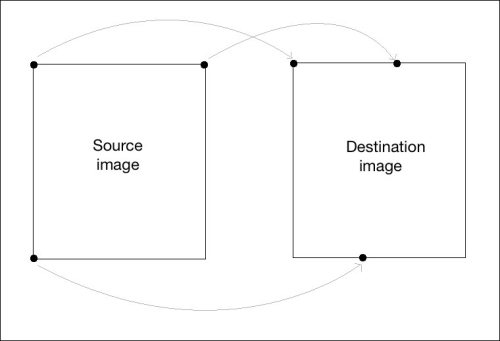
\includegraphics[width=0.6\columnwidth]{figures/Fig25.png}
	\caption{Affine Transformation}
	\label{fig25}
\end{figure}

To get the transformation matrix, we have a function called \textbf{getAffineTransform} in OpenCV. Once we have the affine 	transformation matrix, we use the \textbf{warpAffine} function to apply this matrix to the input image. We can also get the 	mirror image of the input image. We just need to change the control points in the following way:

\vspace{0.5cm}

\begin{tcolorbox}[breakable, size=fbox, boxrule=1pt, pad at break*=1mm,colback=cellbackground, colframe=cellborder]
	\prompt{In}{incolor}{ }{\boxspacing}
	\begin{Verbatim}[commandchars=\\\{\}]
\PY{k+kn}{import} \PY{n+nn}{cv2}
\PY{k+kn}{import} \PY{n+nn}{numpy} \PY{k}{as} \PY{n+nn}{np}
\PY{k+kn}{import} \PY{n+nn}{matplotlib}\PY{n+nn}{.}\PY{n+nn}{pyplot} \PY{k}{as} \PY{n+nn}{plt}
	\end{Verbatim}
\end{tcolorbox}

\begin{tcolorbox}[breakable, size=fbox, boxrule=1pt, pad at break*=1mm,colback=cellbackground, colframe=cellborder]
	\prompt{In}{incolor}{ }{\boxspacing}
	\begin{Verbatim}[commandchars=\\\{\}]
\PY{n}{img} \PY{o}{=} \PY{n}{cv2}\PY{o}{.}\PY{n}{imread}\PY{p}{(}\PY{l+s+s1}{\PYZsq{}}\PY{l+s+s1}{images/Sample7.jpg}\PY{l+s+s1}{\PYZsq{}}\PY{p}{)}
\PY{n}{rows}\PY{p}{,} \PY{n}{cols} \PY{o}{=} \PY{n}{img}\PY{o}{.}\PY{n}{shape}\PY{p}{[}\PY{p}{:}\PY{l+m+mi}{2}\PY{p}{]}
		
\PY{n+nb}{print}\PY{p}{(}\PY{l+s+s1}{\PYZsq{}}\PY{l+s+s1}{rows : }\PY{l+s+si}{\PYZob{}\PYZcb{}}\PY{l+s+s1}{\PYZsq{}}\PY{o}{.}\PY{n}{format}\PY{p}{(}\PY{n}{rows}\PY{p}{)}\PY{p}{)}
\PY{n+nb}{print}\PY{p}{(}\PY{l+s+s1}{\PYZsq{}}\PY{l+s+s1}{columns : }\PY{l+s+si}{\PYZob{}\PYZcb{}}\PY{l+s+s1}{\PYZsq{}}\PY{o}{.}\PY{n}{format}\PY{p}{(}\PY{n}{cols}\PY{p}{)}\PY{p}{)}
	\end{Verbatim}
\end{tcolorbox}

\begin{Verbatim}[commandchars=\\\{\}]
rows : 299
columns : 299
\end{Verbatim}


\begin{tcolorbox}[breakable, size=fbox, boxrule=1pt, pad at break*=1mm,colback=cellbackground, colframe=cellborder]
	\prompt{In}{incolor}{ }{\boxspacing}
	\begin{Verbatim}[commandchars=\\\{\}]
\PY{n}{src\PYZus{}points} \PY{o}{=} \PY{n}{np}\PY{o}{.}\PY{n}{float32}\PY{p}{(}\PY{p}{[}\PY{p}{[}\PY{l+m+mi}{0}\PY{p}{,}\PY{l+m+mi}{0}\PY{p}{]}\PY{p}{,} \PY{p}{[}\PY{n}{cols}\PY{o}{\PYZhy{}}\PY{l+m+mi}{1}\PY{p}{,}\PY{l+m+mi}{0}\PY{p}{]}\PY{p}{,} \PY{p}{[}\PY{l+m+mi}{0}\PY{p}{,}\PY{n}{rows}\PY{o}{\PYZhy{}}\PY{l+m+mi}{1}\PY{p}{]}\PY{p}{]}\PY{p}{)}
\PY{n}{dst\PYZus{}points} \PY{o}{=} \PY{n}{np}\PY{o}{.}\PY{n}{float32}\PY{p}{(}\PY{p}{[}\PY{p}{[}\PY{n}{cols}\PY{o}{\PYZhy{}}\PY{l+m+mi}{1}\PY{p}{,}\PY{l+m+mi}{0}\PY{p}{]}\PY{p}{,} \PY{p}{[}\PY{l+m+mi}{0}\PY{p}{,}\PY{l+m+mi}{0}\PY{p}{]}\PY{p}{,} \PY{p}{[}\PY{n}{cols}\PY{o}{\PYZhy{}}\PY{l+m+mi}{1}\PY{p}{,}\PY{n}{rows}\PY{o}{\PYZhy{}}\PY{l+m+mi}{1}\PY{p}{]}\PY{p}{]}\PY{p}{)}

\PY{n+nb}{print}\PY{p}{(}\PY{l+s+s1}{\PYZsq{}}\PY{l+s+s1}{Source points:}\PY{l+s+se}{\PYZbs{}n}\PY{l+s+s1}{ }\PY{l+s+si}{\PYZob{}\PYZcb{}}\PY{l+s+s1}{\PYZsq{}}\PY{o}{.}\PY{n}{format}\PY{p}{(}\PY{n}{src\PYZus{}points}\PY{p}{)}\PY{p}{)}
\PY{n+nb}{print}\PY{p}{(}\PY{l+s+s1}{\PYZsq{}}\PY{l+s+s1}{Destination Points:}\PY{l+s+se}{\PYZbs{}n}\PY{l+s+s1}{ }\PY{l+s+si}{\PYZob{}\PYZcb{}}\PY{l+s+s1}{\PYZsq{}}\PY{o}{.}\PY{n}{format}\PY{p}{(}\PY{n}{dst\PYZus{}points}\PY{p}{)}\PY{p}{)}
	\end{Verbatim}
\end{tcolorbox}

\begin{Verbatim}[commandchars=\\\{\}]
Source points:
[  0.   0.]
[298.   0.]
[  0. 298.]
Destination Points:
[298.   0.]
[  0.   0.]
[298. 298.]
\end{Verbatim}

\begin{tcolorbox}[breakable, size=fbox, boxrule=1pt, pad at break*=1mm,colback=cellbackground, colframe=cellborder]
	\prompt{In}{incolor}{ }{\boxspacing}
	\begin{Verbatim}[commandchars=\\\{\}]
\PY{n}{affine\PYZus{}matrix} \PY{o}{=} \PY{n}{cv2}\PY{o}{.}\PY{n}{getAffineTransform}\PY{p}{(}\PY{n}{src\PYZus{}points}\PY{p}{,} \PY{n}{dst\PYZus{}points}\PY{p}{)}
\PY{n}{img\PYZus{}output} \PY{o}{=} \PY{n}{cv2}\PY{o}{.}\PY{n}{warpAffine}\PY{p}{(}\PY{n}{img}\PY{p}{,} \PY{n}{affine\PYZus{}matrix}\PY{p}{,} \PY{p}{(}\PY{n}{cols}\PY{p}{,}\PY{n}{rows}\PY{p}{)}\PY{p}{)}
	\end{Verbatim}
\end{tcolorbox}

\begin{tcolorbox}[breakable, size=fbox, boxrule=1pt, pad at break*=1mm,colback=cellbackground, colframe=cellborder]
	\prompt{In}{incolor}{ }{\boxspacing}
	\begin{Verbatim}[commandchars=\\\{\}]
\PY{n}{fig}\PY{p}{,} \PY{n}{axs} \PY{o}{=} \PY{n}{plt}\PY{o}{.}\PY{n}{subplots}\PY{p}{(}\PY{l+m+mi}{1}\PY{p}{,}\PY{l+m+mi}{2}\PY{p}{,}\PY{n}{figsize}\PY{o}{=}\PY{p}{(}\PY{l+m+mi}{10}\PY{p}{,}\PY{l+m+mi}{5}\PY{p}{)}\PY{p}{)}

\PY{n}{axs}\PY{p}{[}\PY{l+m+mi}{0}\PY{p}{]}\PY{o}{.}\PY{n}{imshow}\PY{p}{(}\PY{n}{img}\PY{p}{)}
\PY{n}{axs}\PY{p}{[}\PY{l+m+mi}{0}\PY{p}{]}\PY{o}{.}\PY{n}{set\PYZus{}title}\PY{p}{(}\PY{l+s+s1}{\PYZsq{}}\PY{l+s+s1}{Input}\PY{l+s+s1}{\PYZsq{}}\PY{p}{)}
\PY{n}{axs}\PY{p}{[}\PY{l+m+mi}{1}\PY{p}{]}\PY{o}{.}\PY{n}{imshow}\PY{p}{(}\PY{n}{img\PYZus{}output}\PY{p}{)}
\PY{n}{axs}\PY{p}{[}\PY{l+m+mi}{1}\PY{p}{]}\PY{o}{.}\PY{n}{set\PYZus{}title}\PY{p}{(}\PY{l+s+s1}{\PYZsq{}}\PY{l+s+s1}{Output}\PY{l+s+s1}{\PYZsq{}}\PY{p}{)}
	\end{Verbatim}
\end{tcolorbox}

\begin{tcolorbox}[breakable, size=fbox, boxrule=.5pt, pad at break*=1mm, opacityfill=0]
	\prompt{Out}{outcolor}{ }{\boxspacing}
	\begin{Verbatim}[commandchars=\\\{\}]
Text(0.5, 1.0, 'Output')
	\end{Verbatim}
\end{tcolorbox}

\begin{center}
	\adjustimage{max size={0.9\linewidth}{0.9\paperheight}}{figures/p9.png}
\end{center}
{ \hspace*{\fill} \\}

Here, the mapping looks something like this(Figure \ref{fig26}):

\begin{figure}[H]
	%\resizebox{\linewidth}{!}{
	\centering 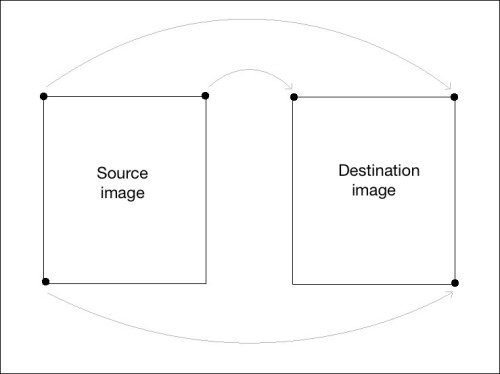
\includegraphics[width=0.6\columnwidth]{figures/Fig26.jpg}
	\caption{Affine Transformation}
	\label{fig26}
\end{figure}

\subsection{Projective Transformations}
Affine transformations are useful, but they impose certain restrictions. A projective transformation, on the other hand, gives us more freedom. It is also referred to as \textbf{homography}. In order to understand projective transformations, we need to understand how projective geometry works. We basically describe what happens to an image when the point of view is changed. For example, if you are standing right in front of a sheet of paper with a square drawn on it, it will look like a square. Now, if you start tilting that sheet of paper, the square will start looking more and more like a trapezoid. Projective transformations allow us to capture this dynamic in a nice mathematical way. These transformations preserve neither sizes nor angles, but they do preserve incidence and cross-ratio.

We can say that any two images on a given plane are related by a homography. As long as they are in the same plane, we can transform anything into anything else. This has many practical applications such as augmented reality, image rectification, image registration, or the computation of camera motion between two images. Once the camera rotation and translation have been extracted from an estimated homography matrix, this information may be used for navigation, or to insert models of 3D objects into an image or video. This way, they are rendered with the correct perspective and it will look like they were part of the original scene.

\vspace{0.5cm}

 \begin{tcolorbox}[breakable, size=fbox, boxrule=1pt, pad at break*=1mm,colback=cellbackground, colframe=cellborder]
	\prompt{In}{incolor}{ }{\boxspacing}
	\begin{Verbatim}[commandchars=\\\{\}]
\PY{k+kn}{import} \PY{n+nn}{cv2}
\PY{k+kn}{import} \PY{n+nn}{numpy} \PY{k}{as} \PY{n+nn}{np}
\PY{k+kn}{import} \PY{n+nn}{matplotlib}\PY{n+nn}{.}\PY{n+nn}{pyplot} \PY{k}{as} \PY{n+nn}{plt}
	\end{Verbatim}
\end{tcolorbox}

\begin{tcolorbox}[breakable, size=fbox, boxrule=1pt, pad at break*=1mm,colback=cellbackground, colframe=cellborder]
	\prompt{In}{incolor}{ }{\boxspacing}
	\begin{Verbatim}[commandchars=\\\{\}]
\PY{n}{img} \PY{o}{=} \PY{n}{cv2}\PY{o}{.}\PY{n}{imread}\PY{p}{(}\PY{l+s+s1}{\PYZsq{}}\PY{l+s+s1}{images/Sample8.jpg}\PY{l+s+s1}{\PYZsq{}}\PY{p}{)}
\PY{n}{rows}\PY{p}{,} \PY{n}{cols} \PY{o}{=} \PY{n}{img}\PY{o}{.}\PY{n}{shape}\PY{p}{[}\PY{p}{:}\PY{l+m+mi}{2}\PY{p}{]}

\PY{n+nb}{print}\PY{p}{(}\PY{l+s+s1}{\PYZsq{}}\PY{l+s+s1}{Rows: }\PY{l+s+si}{\PYZob{}\PYZcb{}}\PY{l+s+s1}{\PYZsq{}}\PY{o}{.}\PY{n}{format}\PY{p}{(}\PY{n}{rows}\PY{p}{)}\PY{p}{)}
\PY{n+nb}{print}\PY{p}{(}\PY{l+s+s1}{\PYZsq{}}\PY{l+s+s1}{Columns: }\PY{l+s+si}{\PYZob{}\PYZcb{}}\PY{l+s+s1}{\PYZsq{}}\PY{o}{.}\PY{n}{format}\PY{p}{(}\PY{n}{cols}\PY{p}{)}\PY{p}{)}
	\end{Verbatim}
\end{tcolorbox}

 \begin{Verbatim}[commandchars=\\\{\}]
Rows: 638
Columns: 750
\end{Verbatim}

\begin{tcolorbox}[breakable, size=fbox, boxrule=1pt, pad at break*=1mm,colback=cellbackground, colframe=cellborder]
	\prompt{In}{incolor}{ }{\boxspacing}
	\begin{Verbatim}[commandchars=\\\{\}]
\PY{n}{src\PYZus{}points} \PY{o}{=} \PY{n}{np}\PY{o}{.}\PY{n}{float32}\PY{p}{(}\PY{p}{[}\PY{p}{[}\PY{l+m+mi}{0}\PY{p}{,}\PY{l+m+mi}{0}\PY{p}{]}\PY{p}{,} \PY{p}{[}\PY{n}{cols}\PY{o}{\PYZhy{}}\PY{l+m+mi}{1}\PY{p}{,}\PY{l+m+mi}{0}\PY{p}{]}\PY{p}{,} \PY{p}{[}\PY{l+m+mi}{0}\PY{p}{,}\PY{n}{rows}\PY{o}{\PYZhy{}}\PY{l+m+mi}{1}\PY{p}{]}\PY{p}{,}
\PY{p}{[}\PY{n}{cols}\PY{o}{\PYZhy{}}\PY{l+m+mi}{1}\PY{p}{,}\PY{n}{rows}\PY{o}{\PYZhy{}}\PY{l+m+mi}{1}\PY{p}{]}\PY{p}{]}\PY{p}{)}
\PY{n}{dst\PYZus{}points} \PY{o}{=} \PY{n}{np}\PY{o}{.}\PY{n}{float32}\PY{p}{(}\PY{p}{[}\PY{p}{[}\PY{l+m+mi}{0}\PY{p}{,}\PY{l+m+mi}{0}\PY{p}{]}\PY{p}{,} \PY{p}{[}\PY{n}{cols}\PY{o}{\PYZhy{}}\PY{l+m+mi}{1}\PY{p}{,}\PY{l+m+mi}{0}\PY{p}{]}\PY{p}{,} \PY{p}{[}\PY{n+nb}{int}\PY{p}{(}\PY{l+m+mf}{0.33}\PY{o}{*}\PY{n}{cols}\PY{p}{)}\PY{p}{,}\PY{n}{rows}\PY{o}{\PYZhy{}}\PY{l+m+mi}{1}\PY{p}{]}\PY{p}{,}
\PY{p}{[}\PY{n+nb}{int}\PY{p}{(}\PY{l+m+mf}{0.66}\PY{o}{*}\PY{n}{cols}\PY{p}{)}\PY{p}{,}\PY{n}{rows}\PY{o}{\PYZhy{}}\PY{l+m+mi}{1}\PY{p}{]}\PY{p}{]}\PY{p}{)} 

\PY{n+nb}{print}\PY{p}{(}\PY{l+s+s1}{\PYZsq{}}\PY{l+s+s1}{Source points:}\PY{l+s+se}{\PYZbs{}n}\PY{l+s+s1}{ }\PY{l+s+si}{\PYZob{}\PYZcb{}}\PY{l+s+s1}{\PYZsq{}}\PY{o}{.}\PY{n}{format}\PY{p}{(}\PY{n}{src\PYZus{}points}\PY{p}{)}\PY{p}{)}
\PY{n+nb}{print}\PY{p}{(}\PY{l+s+s1}{\PYZsq{}}\PY{l+s+s1}{Destination points:}\PY{l+s+se}{\PYZbs{}n}\PY{l+s+s1}{ }\PY{l+s+si}{\PYZob{}\PYZcb{}}\PY{l+s+s1}{\PYZsq{}}\PY{o}{.}\PY{n}{format}\PY{p}{(}\PY{n}{dst\PYZus{}points}\PY{p}{)}\PY{p}{)}
	\end{Verbatim}
\end{tcolorbox}

\begin{Verbatim}[commandchars=\\\{\}]
Source points:
[  0.   0.]
[749.   0.]
[  0. 637.]
[749. 637.]
Destination points:
[  0.   0.]
[749.   0.]
[247. 637.]
[495. 637.]
\end{Verbatim}

\begin{tcolorbox}[breakable, size=fbox, boxrule=1pt, pad at break*=1mm,colback=cellbackground, colframe=cellborder]
	\prompt{In}{incolor}{ }{\boxspacing}
	\begin{Verbatim}[commandchars=\\\{\}]
\PY{n}{projective\PYZus{}matrix} \PY{o}{=} \PY{n}{cv2}\PY{o}{.}\PY{n}{getPerspectiveTransform}\PY{p}{(}\PY{n}{src\PYZus{}points}\PY{p}{,} \PY{n}{dst\PYZus{}points}\PY{p}{)}
\PY{n}{img\PYZus{}output} \PY{o}{=} \PY{n}{cv2}\PY{o}{.}\PY{n}{warpPerspective}\PY{p}{(}\PY{n}{img}\PY{p}{,} \PY{n}{projective\PYZus{}matrix}\PY{p}{,} \PY{p}{(}\PY{n}{cols}\PY{p}{,}\PY{n}{rows}\PY{p}{)}\PY{p}{)}
	\end{Verbatim}
\end{tcolorbox}
\vspace{0.5cm}
\begin{tcolorbox}[breakable, size=fbox, boxrule=1pt, pad at break*=1mm,colback=cellbackground, colframe=cellborder]
	\prompt{In}{incolor}{ }{\boxspacing}
	\begin{Verbatim}[commandchars=\\\{\}]
\PY{n}{fig}\PY{p}{,} \PY{n}{axs} \PY{o}{=} \PY{n}{plt}\PY{o}{.}\PY{n}{subplots}\PY{p}{(}\PY{l+m+mi}{1}\PY{p}{,}\PY{l+m+mi}{2}\PY{p}{,}\PY{n}{figsize}\PY{o}{=}\PY{p}{(}\PY{l+m+mi}{10}\PY{p}{,}\PY{l+m+mi}{5}\PY{p}{)}\PY{p}{)}

\PY{n}{axs}\PY{p}{[}\PY{l+m+mi}{0}\PY{p}{]}\PY{o}{.}\PY{n}{imshow}\PY{p}{(}\PY{n}{img}\PY{p}{)}
\PY{n}{axs}\PY{p}{[}\PY{l+m+mi}{0}\PY{p}{]}\PY{o}{.}\PY{n}{set\PYZus{}title}\PY{p}{(}\PY{l+s+s1}{\PYZsq{}}\PY{l+s+s1}{Input}\PY{l+s+s1}{\PYZsq{}}\PY{p}{)}
\PY{n}{axs}\PY{p}{[}\PY{l+m+mi}{1}\PY{p}{]}\PY{o}{.}\PY{n}{imshow}\PY{p}{(}\PY{n}{img\PYZus{}output}\PY{p}{)}
\PY{n}{axs}\PY{p}{[}\PY{l+m+mi}{1}\PY{p}{]}\PY{o}{.}\PY{n}{set\PYZus{}title}\PY{p}{(}\PY{l+s+s1}{\PYZsq{}}\PY{l+s+s1}{Output}\PY{l+s+s1}{\PYZsq{}}\PY{p}{)}
	\end{Verbatim}
\end{tcolorbox}

\begin{tcolorbox}[breakable, size=fbox, boxrule=.5pt, pad at break*=1mm, opacityfill=0]
\prompt{Out}{outcolor}{ }{\boxspacing}
\begin{Verbatim}[commandchars=\\\{\}]
Text(0.5, 1.0, 'Output')
\end{Verbatim}
\end{tcolorbox}

\begin{center}
	\adjustimage{max size={0.9\linewidth}{0.9\paperheight}}{figures/p10.png}
\end{center}
{ \hspace*{\fill} \\}

We can choose four control points in the source image and map them to the destination image. Parallel lines will not remain parallel lines after the transformation. We use a function called \textbf{getPerspectiveTransform} to get the transformation matrix.


\section{Image Filters}

In this section, we will learn how to use fundamental image processing operators. We are going to discuss edge detection and how we can use image filters to apply various effects on photos.

\subsection{2D Convolution}
Convolution is a fundamental operation in image processing. We basically apply a mathematical operator to each pixel and change its value in some way. To apply this mathematical operator, we use another matrix called a kernel. The kernel is usually much smaller in size than the input image. For each pixel in the image, we take the kernel and place it on top such that the center of the kernel coincides with the pixel under consideration. We then multiply each value in the kernel matrix with the corresponding values in the image, and then sum it up. This is the new value that will be substituted in this position in the output image.

Here, the kernel is called the \textbf{image filter} and the process of applying this kernel to the given image is called \textbf{image filtering}. The output obtained after applying the kernel to the image is called the filtered image. Depending on the values in the kernel, it performs different functions like blurring, detecting edges, and so on. Figure \ref{fig27} should help you visualize the image filtering operation:

\begin{figure}[H]
	%\resizebox{\linewidth}{!}{
	\centering 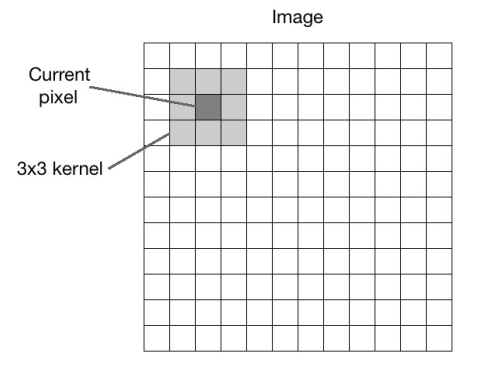
\includegraphics[width=0.6\columnwidth]{figures/Fig27.png}
	\caption{Image Kernel}
	\label{fig27}
\end{figure}

Let's start with the simplest case which is identity kernel. This kernel doesn't really change the input image. If we consider a 3$\times$3 identity kernel, it looks something like the following:

\begin{center}
	\[
	\textit{I} =  
	\begin{bmatrix}
		0 & 0 & 0 \\
		0 & 1 & 0 \\
		0 & 0 & 0
	\end{bmatrix}
	\]
\end{center}

\subsection{Blurring}
Blurring refers to averaging the pixel values within a neighborhood. This is also called a \textbf{low pass filter}. A low pass filter is a filter that allows low frequencies and blocks higher frequencies. Frequency refers to the rate of change of pixel values. So we can say that the sharp edges would be high frequency content because the pixel values change rapidly in that region. Going by that logic, plain areas would be low frequency content. Going by this definition, a low pass filter would try to smoothen the edges.

A simple way to build a low pass filter is by uniformly averaging the values in the neighborhood of a pixel. We can choose the size of the kernel depending on how much we want to smoothen the image, and it will correspondingly have different effects. If you choose a bigger size, then you will be averaging over a larger area. This tends to increase the smoothening effect. A 3$\times$3 low pass filter kernel looks like the following:

\begin{center}
	\[
	\textit{I} = \frac{1}{9}  
	\begin{bmatrix}
		1 & 1 & 1 \\
		1 & 1 & 1 \\
		1 & 1 & 1
	\end{bmatrix}
	\]
\end{center}

We are dividing the matrix by 9 because we want the values to sum up to 1. This is called \textbf{normalization}, and it's important because we don't want to artificially increase the intensity value at that pixel's location. So you should normalize the kernel before applying it to an image. Here is the code to apply this low pass filter to an image:

\vspace{0.5cm}

\begin{tcolorbox}[breakable, size=fbox, boxrule=1pt, pad at break*=1mm,colback=cellbackground, colframe=cellborder]
	\prompt{In}{incolor}{ }{\boxspacing}
	\begin{Verbatim}[commandchars=\\\{\}]
\PY{k+kn}{import} \PY{n+nn}{cv2}
\PY{k+kn}{import} \PY{n+nn}{numpy} \PY{k}{as} \PY{n+nn}{np}
\PY{k+kn}{import} \PY{n+nn}{matplotlib}\PY{n+nn}{.}\PY{n+nn}{pyplot} \PY{k}{as} \PY{n+nn}{plt}
	\end{Verbatim}
\end{tcolorbox}

\begin{tcolorbox}[breakable, size=fbox, boxrule=1pt, pad at break*=1mm,colback=cellbackground, colframe=cellborder]
	\prompt{In}{incolor}{ }{\boxspacing}
	\begin{Verbatim}[commandchars=\\\{\}]
\PY{n}{img} \PY{o}{=} \PY{n}{cv2}\PY{o}{.}\PY{n}{imread}\PY{p}{(}\PY{l+s+s1}{\PYZsq{}}\PY{l+s+s1}{images/Sample9.jpg}\PY{l+s+s1}{\PYZsq{}}\PY{p}{)}
\PY{n}{rows}\PY{p}{,} \PY{n}{cols} \PY{o}{=} \PY{n}{img}\PY{o}{.}\PY{n}{shape}\PY{p}{[}\PY{p}{:}\PY{l+m+mi}{2}\PY{p}{]}

\PY{n+nb}{print}\PY{p}{(}\PY{l+s+s1}{\PYZsq{}}\PY{l+s+s1}{Rows: }\PY{l+s+si}{\PYZob{}\PYZcb{}}\PY{l+s+s1}{\PYZsq{}}\PY{o}{.}\PY{n}{format}\PY{p}{(}\PY{n}{rows}\PY{p}{)}\PY{p}{)}
\PY{n+nb}{print}\PY{p}{(}\PY{l+s+s1}{\PYZsq{}}\PY{l+s+s1}{Columns: }\PY{l+s+si}{\PYZob{}\PYZcb{}}\PY{l+s+s1}{\PYZsq{}}\PY{o}{.}\PY{n}{format}\PY{p}{(}\PY{n}{cols}\PY{p}{)}\PY{p}{)}
	\end{Verbatim}
\end{tcolorbox}

\begin{Verbatim}[commandchars=\\\{\}]
Rows: 765
Columns: 637
\end{Verbatim}

\begin{tcolorbox}[breakable, size=fbox, boxrule=1pt, pad at break*=1mm,colback=cellbackground, colframe=cellborder]
	\prompt{In}{incolor}{ }{\boxspacing}
	\begin{Verbatim}[commandchars=\\\{\}]
\PY{c+c1}{\PYZsh{} Create Kernels}
\PY{n}{kernel\PYZus{}identity} \PY{o}{=} \PY{n}{np}\PY{o}{.}\PY{n}{array}\PY{p}{(}\PY{p}{[}\PY{p}{[}\PY{l+m+mi}{0}\PY{p}{,}\PY{l+m+mi}{0}\PY{p}{,}\PY{l+m+mi}{0}\PY{p}{]}\PY{p}{,} \PY{p}{[}\PY{l+m+mi}{0}\PY{p}{,}\PY{l+m+mi}{1}\PY{p}{,}\PY{l+m+mi}{0}\PY{p}{]}\PY{p}{,} \PY{p}{[}\PY{l+m+mi}{0}\PY{p}{,}\PY{l+m+mi}{0}\PY{p}{,}\PY{l+m+mi}{0}\PY{p}{]}\PY{p}{]}\PY{p}{)}
\PY{n}{kernel\PYZus{}5x5} \PY{o}{=} \PY{n}{np}\PY{o}{.}\PY{n}{ones}\PY{p}{(}\PY{p}{(}\PY{l+m+mi}{5}\PY{p}{,}\PY{l+m+mi}{5}\PY{p}{)}\PY{p}{,} \PY{n}{np}\PY{o}{.}\PY{n}{float32}\PY{p}{)} \PY{o}{/} \PY{l+m+mf}{25.0}
\PY{n}{kernel\PYZus{}9x9} \PY{o}{=} \PY{n}{np}\PY{o}{.}\PY{n}{ones}\PY{p}{(}\PY{p}{(}\PY{l+m+mi}{9}\PY{p}{,}\PY{l+m+mi}{9}\PY{p}{)}\PY{p}{,} \PY{n}{np}\PY{o}{.}\PY{n}{float32}\PY{p}{)} \PY{o}{/} \PY{l+m+mf}{81.0}
	\end{Verbatim}
\end{tcolorbox}

\begin{tcolorbox}[breakable, size=fbox, boxrule=1pt, pad at break*=1mm,colback=cellbackground, colframe=cellborder]
	\prompt{In}{incolor}{ }{\boxspacing}
	\begin{Verbatim}[commandchars=\\\{\}]
\PY{c+c1}{\PYZsh{} Apply Kernels}
\PY{n}{identity\PYZus{}img} \PY{o}{=} \PY{n}{cv2}\PY{o}{.}\PY{n}{filter2D}\PY{p}{(}\PY{n}{img}\PY{p}{,} \PY{o}{\PYZhy{}}\PY{l+m+mi}{1}\PY{p}{,} \PY{n}{kernel\PYZus{}identity}\PY{p}{)}
\PY{n}{kernel\PYZus{}5x5\PYZus{}img} \PY{o}{=} \PY{n}{cv2}\PY{o}{.}\PY{n}{filter2D}\PY{p}{(}\PY{n}{img}\PY{p}{,} \PY{o}{\PYZhy{}}\PY{l+m+mi}{1}\PY{p}{,} \PY{n}{kernel\PYZus{}5x5}\PY{p}{)}
\PY{n}{kernel\PYZus{}9x9\PYZus{}img} \PY{o}{=} \PY{n}{cv2}\PY{o}{.}\PY{n}{filter2D}\PY{p}{(}\PY{n}{img}\PY{p}{,} \PY{o}{\PYZhy{}}\PY{l+m+mi}{1}\PY{p}{,} \PY{n}{kernel\PYZus{}9x9}\PY{p}{)}
	\end{Verbatim}
\end{tcolorbox}

\begin{tcolorbox}[breakable, size=fbox, boxrule=1pt, pad at break*=1mm,colback=cellbackground, colframe=cellborder]
	\prompt{In}{incolor}{ }{\boxspacing}
	\begin{Verbatim}[commandchars=\\\{\}]
\PY{n}{fig}\PY{p}{,} \PY{n}{axs} \PY{o}{=} \PY{n}{plt}\PY{o}{.}\PY{n}{subplots}\PY{p}{(}\PY{l+m+mi}{2}\PY{p}{,}\PY{l+m+mi}{2}\PY{p}{,}\PY{n}{figsize}\PY{o}{=}\PY{p}{(}\PY{l+m+mi}{10}\PY{p}{,}\PY{l+m+mi}{10}\PY{p}{)}\PY{p}{)}

\PY{n}{axs}\PY{p}{[}\PY{l+m+mi}{0}\PY{p}{,}\PY{l+m+mi}{0}\PY{p}{]}\PY{o}{.}\PY{n}{imshow}\PY{p}{(}\PY{n}{img}\PY{p}{)}
\PY{n}{axs}\PY{p}{[}\PY{l+m+mi}{0}\PY{p}{,}\PY{l+m+mi}{0}\PY{p}{]}\PY{o}{.}\PY{n}{set\PYZus{}title}\PY{p}{(}\PY{l+s+s1}{\PYZsq{}}\PY{l+s+s1}{Input}\PY{l+s+s1}{\PYZsq{}}\PY{p}{)}

\PY{n}{axs}\PY{p}{[}\PY{l+m+mi}{0}\PY{p}{,}\PY{l+m+mi}{1}\PY{p}{]}\PY{o}{.}\PY{n}{imshow}\PY{p}{(}\PY{n}{identity\PYZus{}img}\PY{p}{)}
\PY{n}{axs}\PY{p}{[}\PY{l+m+mi}{0}\PY{p}{,}\PY{l+m+mi}{1}\PY{p}{]}\PY{o}{.}\PY{n}{set\PYZus{}title}\PY{p}{(}\PY{l+s+s1}{\PYZsq{}}\PY{l+s+s1}{identity kernel}\PY{l+s+s1}{\PYZsq{}}\PY{p}{)}

\PY{n}{axs}\PY{p}{[}\PY{l+m+mi}{1}\PY{p}{,}\PY{l+m+mi}{0}\PY{p}{]}\PY{o}{.}\PY{n}{imshow}\PY{p}{(}\PY{n}{kernel\PYZus{}5x5\PYZus{}img}\PY{p}{)}
\PY{n}{axs}\PY{p}{[}\PY{l+m+mi}{1}\PY{p}{,}\PY{l+m+mi}{0}\PY{p}{]}\PY{o}{.}\PY{n}{set\PYZus{}title}\PY{p}{(}\PY{l+s+s1}{\PYZsq{}}\PY{l+s+s1}{5x5 kernel}\PY{l+s+s1}{\PYZsq{}}\PY{p}{)}

\PY{n}{axs}\PY{p}{[}\PY{l+m+mi}{1}\PY{p}{,}\PY{l+m+mi}{1}\PY{p}{]}\PY{o}{.}\PY{n}{imshow}\PY{p}{(}\PY{n}{kernel\PYZus{}9x9\PYZus{}img}\PY{p}{)}
\PY{n}{axs}\PY{p}{[}\PY{l+m+mi}{1}\PY{p}{,}\PY{l+m+mi}{1}\PY{p}{]}\PY{o}{.}\PY{n}{set\PYZus{}title}\PY{p}{(}\PY{l+s+s1}{\PYZsq{}}\PY{l+s+s1}{9x9 kernel}\PY{l+s+s1}{\PYZsq{}}\PY{p}{)}
	\end{Verbatim}
\end{tcolorbox}

\begin{tcolorbox}[breakable, size=fbox, boxrule=.5pt, pad at break*=1mm, opacityfill=0]
	\prompt{Out}{outcolor}{ }{\boxspacing}
	\begin{Verbatim}[commandchars=\\\{\}]
Text(0.5, 1.0, '9x9 kernel')
	\end{Verbatim}
\end{tcolorbox}

\begin{center}
	\adjustimage{max size={0.9\linewidth}{0.9\paperheight}}{figures/p11.png}
\end{center}
{ \hspace*{\fill} \\}

In the preceding code, we are generating different kernels in the code which are kernel\_identity, kernel\_5$\times$5, and kernel\_9$\times$9. We use the function, \textbf{filter2D}, to apply these kernels to the input image. If you look at the images carefully, you can see that they keep getting blurrier as we increase the kernel size. The reason for this is because when we increase the kernel size, we are averaging over a larger area. This tends to have a larger blurring effect. An alternative way of doing this would be by using the OpenCV function, \textbf{cv2.blur}. If you don't want to generate the kernels yourself, you can just use this function directly.

\section{Edge Detection}
The process of edge detection involves detecting sharp edges in the image and producing a binary image as the output. Typically, we draw white lines on a black background to indicate those edges. We can think of edge detection as a high pass filtering operation. A high pass filter allows high frequency content to pass through and blocks the low frequency content. As we discussed earlier, edges are high frequency content. In edge detection, we want to retain these edges and discard everything else. Hence, we should build a kernel that is the equivalent of a high pass filter.

Let's start with a simple edge detection filter known as the Sobel filter. Since edges can occur in both horizontal and vertical directions, the \textbf{Sobel filter} is composed of the following two kernels:

\begin{center}
	\[
	\textit{$S_x$} =  
	\begin{bmatrix}
		-1 & 0 & 1 \\
		-2 & 1 & 2 \\
		-1 & 0 & 1
	\end{bmatrix}
	\]
	\hspace{2cm}
	\[
	\textit{$S_y$} =  
	\begin{bmatrix}
		-1 & -2 & -1 \\
		0 & 0 & 0 \\
		1 & 2 & 1
	\end{bmatrix}
	\]
\end{center}

The kernel on the left detects horizontal edges and the kernel on the right detects vertical edges. OpenCV provides a function to directly apply the Sobel filter to a given image.

\vspace{0.5cm}

\begin{tcolorbox}[breakable, size=fbox, boxrule=1pt, pad at break*=1mm,colback=cellbackground, colframe=cellborder]
	\prompt{In}{incolor}{ }{\boxspacing}
	\begin{Verbatim}[commandchars=\\\{\}]
\PY{k+kn}{import} \PY{n+nn}{cv2}
\PY{k+kn}{import} \PY{n+nn}{numpy} \PY{k}{as} \PY{n+nn}{np}
\PY{k+kn}{import} \PY{n+nn}{matplotlib}\PY{n+nn}{.}\PY{n+nn}{pyplot} \PY{k}{as} \PY{n+nn}{plt}
	\end{Verbatim}
\end{tcolorbox}

\begin{tcolorbox}[breakable, size=fbox, boxrule=1pt, pad at break*=1mm,colback=cellbackground, colframe=cellborder]
	\prompt{In}{incolor}{10}{\boxspacing}
	\begin{Verbatim}[commandchars=\\\{\}]
\PY{n}{img} \PY{o}{=} \PY{n}{cv2}\PY{o}{.}\PY{n}{imread}\PY{p}{(}\PY{l+s+s1}{\PYZsq{}}\PY{l+s+s1}{images/Sample10.jpg}\PY{l+s+s1}{\PYZsq{}}\PY{p}{)}
\PY{n}{rows}\PY{p}{,} \PY{n}{cols}\PY{p}{,} \PY{n}{\PYZus{}} \PY{o}{=} \PY{n}{img}\PY{o}{.}\PY{n}{shape}

\PY{n+nb}{print}\PY{p}{(}\PY{l+s+s1}{\PYZsq{}}\PY{l+s+s1}{Rows: }\PY{l+s+si}{\PYZob{}\PYZcb{}}\PY{l+s+s1}{\PYZsq{}}\PY{o}{.}\PY{n}{format}\PY{p}{(}\PY{n}{rows}\PY{p}{)}\PY{p}{)}
\PY{n+nb}{print}\PY{p}{(}\PY{l+s+s1}{\PYZsq{}}\PY{l+s+s1}{Columns: }\PY{l+s+si}{\PYZob{}\PYZcb{}}\PY{l+s+s1}{\PYZsq{}}\PY{o}{.}\PY{n}{format}\PY{p}{(}\PY{n}{cols}\PY{p}{)}\PY{p}{)}
	\end{Verbatim}
\end{tcolorbox}

\begin{Verbatim}[commandchars=\\\{\}]
Rows: 212
Columns: 220
\end{Verbatim}

\begin{tcolorbox}[breakable, size=fbox, boxrule=1pt, pad at break*=1mm,colback=cellbackground, colframe=cellborder]
	\prompt{In}{incolor}{ }{\boxspacing}
	\begin{Verbatim}[commandchars=\\\{\}]
\PY{c+c1}{\PYZsh{} iameg resizing}
\PY{n}{img} \PY{o}{=} \PY{n}{cv2}\PY{o}{.}\PY{n}{resize}\PY{p}{(}\PY{n}{img}\PY{p}{,}\PY{p}{(}\PY{l+m+mi}{400}\PY{p}{,}\PY{l+m+mi}{400}\PY{p}{)}\PY{p}{)}
\PY{n}{rows}\PY{p}{,} \PY{n}{cols}\PY{p}{,}\PY{n}{\PYZus{}} \PY{o}{=} \PY{n}{img}\PY{o}{.}\PY{n}{shape}

\PY{n+nb}{print}\PY{p}{(}\PY{l+s+s1}{\PYZsq{}}\PY{l+s+s1}{Rows: }\PY{l+s+si}{\PYZob{}\PYZcb{}}\PY{l+s+s1}{ }\PY{l+s+se}{\PYZbs{}n}\PY{l+s+s1}{Columns: }\PY{l+s+si}{\PYZob{}\PYZcb{}}\PY{l+s+s1}{\PYZsq{}}\PY{o}{.}\PY{n}{format}\PY{p}{(}\PY{n}{rows}\PY{p}{,}\PY{n}{cols}\PY{p}{)}\PY{p}{)}
	\end{Verbatim}
\end{tcolorbox}

\begin{Verbatim}[commandchars=\\\{\}]
Rows: 400
Columns: 400
\end{Verbatim}

\begin{tcolorbox}[breakable, size=fbox, boxrule=1pt, pad at break*=1mm,colback=cellbackground, colframe=cellborder]
	\prompt{In}{incolor}{ }{\boxspacing}
	\begin{Verbatim}[commandchars=\\\{\}]
\PY{c+c1}{\PYZsh{} create Sobel Kernels}
\PY{n}{sobel\PYZus{}horizontal} \PY{o}{=} \PY{n}{cv2}\PY{o}{.}\PY{n}{Sobel}\PY{p}{(}\PY{n}{img}\PY{p}{,} \PY{n}{cv2}\PY{o}{.}\PY{n}{CV\PYZus{}64F}\PY{p}{,} \PY{l+m+mi}{1}\PY{p}{,} \PY{l+m+mi}{0}\PY{p}{,} \PY{n}{ksize}\PY{o}{=}\PY{l+m+mi}{5}\PY{p}{)}
\PY{n}{sobel\PYZus{}vertical} \PY{o}{=} \PY{n}{cv2}\PY{o}{.}\PY{n}{Sobel}\PY{p}{(}\PY{n}{img}\PY{p}{,} \PY{n}{cv2}\PY{o}{.}\PY{n}{CV\PYZus{}64F}\PY{p}{,} \PY{l+m+mi}{0}\PY{p}{,} \PY{l+m+mi}{1}\PY{p}{,} \PY{n}{ksize}\PY{o}{=}\PY{l+m+mi}{5}\PY{p}{)}
	\end{Verbatim}
\end{tcolorbox}

\begin{tcolorbox}[breakable, size=fbox, boxrule=1pt, pad at break*=1mm,colback=cellbackground, colframe=cellborder]
	\prompt{In}{incolor}{ }{\boxspacing}
	\begin{Verbatim}[commandchars=\\\{\}]
\PY{n}{fig}\PY{p}{,} \PY{n}{axs} \PY{o}{=} \PY{n}{plt}\PY{o}{.}\PY{n}{subplots}\PY{p}{(}\PY{l+m+mi}{1}\PY{p}{,}\PY{l+m+mi}{3}\PY{p}{,}\PY{n}{figsize}\PY{o}{=}\PY{p}{(}\PY{l+m+mi}{15}\PY{p}{,}\PY{l+m+mi}{5}\PY{p}{)}\PY{p}{)}

\PY{n}{axs}\PY{p}{[}\PY{l+m+mi}{0}\PY{p}{]}\PY{o}{.}\PY{n}{imshow}\PY{p}{(}\PY{n}{img}\PY{p}{)}
\PY{n}{axs}\PY{p}{[}\PY{l+m+mi}{0}\PY{p}{]}\PY{o}{.}\PY{n}{set\PYZus{}title}\PY{p}{(}\PY{l+s+s1}{\PYZsq{}}\PY{l+s+s1}{Original}\PY{l+s+s1}{\PYZsq{}}\PY{p}{)}

\PY{n}{axs}\PY{p}{[}\PY{l+m+mi}{1}\PY{p}{]}\PY{o}{.}\PY{n}{imshow}\PY{p}{(}\PY{n}{sobel\PYZus{}horizontal}\PY{p}{)}
\PY{n}{axs}\PY{p}{[}\PY{l+m+mi}{1}\PY{p}{]}\PY{o}{.}\PY{n}{set\PYZus{}title}\PY{p}{(}\PY{l+s+s1}{\PYZsq{}}\PY{l+s+s1}{Sobel horizontal}\PY{l+s+s1}{\PYZsq{}}\PY{p}{)}

\PY{n}{axs}\PY{p}{[}\PY{l+m+mi}{2}\PY{p}{]}\PY{o}{.}\PY{n}{imshow}\PY{p}{(}\PY{n}{sobel\PYZus{}vertical}\PY{p}{)}
\PY{n}{axs}\PY{p}{[}\PY{l+m+mi}{2}\PY{p}{]}\PY{o}{.}\PY{n}{set\PYZus{}title}\PY{p}{(}\PY{l+s+s1}{\PYZsq{}}\PY{l+s+s1}{Sobel vertical}\PY{l+s+s1}{\PYZsq{}}\PY{p}{)}
	\end{Verbatim}
\end{tcolorbox}

\begin{tcolorbox}[breakable, size=fbox, boxrule=.5pt, pad at break*=1mm, opacityfill=0]
	\prompt{Out}{outcolor}{ }{\boxspacing}
	\begin{Verbatim}[commandchars=\\\{\}]
Text(0.5, 1.0, 'Sobel vertical')
	\end{Verbatim}
\end{tcolorbox}

\begin{center}
	\adjustimage{max size={0.9\linewidth}{0.9\paperheight}}{figures/p12.png}
\end{center}
{ \hspace*{\fill} \\}

In the preceding figure, the image in the middle is the output of horizontal edge detector, and the image on the right is the vertical edge detector. As we can see here, the Sobel filter detects edges in either a horizontal or vertical direction and it doesn't give us a holistic view of all the edges. To overcome this, we can use the \textbf{Laplacian filter}. The advantage of using this filter is that it uses double derivative in both directions.

\vspace{0.5cm}

\begin{tcolorbox}[breakable, size=fbox, boxrule=1pt, pad at break*=1mm,colback=cellbackground, colframe=cellborder]
	\prompt{In}{incolor}{ }{\boxspacing}
	\begin{Verbatim}[commandchars=\\\{\}]
\PY{k+kn}{import} \PY{n+nn}{cv2}
\PY{k+kn}{import} \PY{n+nn}{numpy} \PY{k}{as} \PY{n+nn}{np}
\PY{k+kn}{import} \PY{n+nn}{matplotlib}\PY{n+nn}{.}\PY{n+nn}{pyplot} \PY{k}{as} \PY{n+nn}{plt}
	\end{Verbatim}
\end{tcolorbox}

\begin{tcolorbox}[breakable, size=fbox, boxrule=1pt, pad at break*=1mm,colback=cellbackground, colframe=cellborder]
\prompt{In}{incolor}{ }{\boxspacing}
\begin{Verbatim}[commandchars=\\\{\}]
\PY{n}{img} \PY{o}{=} \PY{n}{cv2}\PY{o}{.}\PY{n}{imread}\PY{p}{(}\PY{l+s+s1}{\PYZsq{}}\PY{l+s+s1}{images/Sample11.jpg}\PY{l+s+s1}{\PYZsq{}}\PY{p}{)}
\PY{n}{rows}\PY{p}{,} \PY{n}{cols}\PY{p}{,} \PY{n}{\PYZus{}} \PY{o}{=} \PY{n}{img}\PY{o}{.}\PY{n}{shape}

\PY{n+nb}{print}\PY{p}{(}\PY{l+s+s1}{\PYZsq{}}\PY{l+s+s1}{Rows: }\PY{l+s+si}{\PYZob{}\PYZcb{}}\PY{l+s+s1}{ }\PY{l+s+se}{\PYZbs{}n}\PY{l+s+s1}{Columns: }\PY{l+s+si}{\PYZob{}\PYZcb{}}\PY{l+s+s1}{\PYZsq{}}\PY{o}{.}\PY{n}{format}\PY{p}{(}\PY{n}{rows}\PY{p}{,}\PY{n}{cols}\PY{p}{)}\PY{p}{)}
\end{Verbatim}
\end{tcolorbox}

\begin{Verbatim}[commandchars=\\\{\}]
Rows: 2166
Columns: 2352
\end{Verbatim}

\begin{tcolorbox}[breakable, size=fbox, boxrule=1pt, pad at break*=1mm,colback=cellbackground, colframe=cellborder]
	\prompt{In}{incolor}{ }{\boxspacing}
	\begin{Verbatim}[commandchars=\\\{\}]
\PY{c+c1}{\PYZsh{} apply Laplacian Kernel}
\PY{n}{laplacian} \PY{o}{=} \PY{n}{cv2}\PY{o}{.}\PY{n}{Laplacian}\PY{p}{(}\PY{n}{img}\PY{p}{,} \PY{n}{cv2}\PY{o}{.}\PY{n}{CV\PYZus{}64F}\PY{p}{)}
	\end{Verbatim}
\end{tcolorbox}

\begin{tcolorbox}[breakable, size=fbox, boxrule=1pt, pad at break*=1mm,colback=cellbackground, colframe=cellborder]
	\prompt{In}{incolor}{ }{\boxspacing}
	\begin{Verbatim}[commandchars=\\\{\}]
\PY{n}{fig}\PY{p}{,} \PY{n}{axs} \PY{o}{=} \PY{n}{plt}\PY{o}{.}\PY{n}{subplots}\PY{p}{(}\PY{l+m+mi}{1}\PY{p}{,}\PY{l+m+mi}{2}\PY{p}{,}\PY{n}{figsize}\PY{o}{=}\PY{p}{(}\PY{l+m+mi}{10}\PY{p}{,}\PY{l+m+mi}{5}\PY{p}{)}\PY{p}{)}

\PY{n}{axs}\PY{p}{[}\PY{l+m+mi}{0}\PY{p}{]}\PY{o}{.}\PY{n}{imshow}\PY{p}{(}\PY{n}{img}\PY{p}{)}
\PY{n}{axs}\PY{p}{[}\PY{l+m+mi}{0}\PY{p}{]}\PY{o}{.}\PY{n}{set\PYZus{}title}\PY{p}{(}\PY{l+s+s1}{\PYZsq{}}\PY{l+s+s1}{Original}\PY{l+s+s1}{\PYZsq{}}\PY{p}{)}

\PY{n}{axs}\PY{p}{[}\PY{l+m+mi}{1}\PY{p}{]}\PY{o}{.}\PY{n}{imshow}\PY{p}{(}\PY{n}{laplacian}\PY{p}{)}
\PY{n}{axs}\PY{p}{[}\PY{l+m+mi}{1}\PY{p}{]}\PY{o}{.}\PY{n}{set\PYZus{}title}\PY{p}{(}\PY{l+s+s1}{\PYZsq{}}\PY{l+s+s1}{Laplacian}\PY{l+s+s1}{\PYZsq{}}\PY{p}{)}
	\end{Verbatim}
\end{tcolorbox}


\begin{tcolorbox}[breakable, size=fbox, boxrule=.5pt, pad at break*=1mm, opacityfill=0]
\prompt{Out}{outcolor}{ }{\boxspacing}
\begin{Verbatim}[commandchars=\\\{\}]
Text(0.5, 1.0, 'Laplacian')
\end{Verbatim}
\end{tcolorbox}

\begin{center}
	\adjustimage{max size={0.9\linewidth}{0.9\paperheight}}{figures/p13.png}
\end{center}
{ \hspace*{\fill} \\}

Even though the Laplacian kernel worked in this case, it doesn't always work well. It gives rise to a lot of noise in the output. To overcome this problem, we use the \textbf{Canny edge detector}. To use the Canny edge detector, we can use the following code:

\vspace{0.5cm}

\begin{tcolorbox}[breakable, size=fbox, boxrule=1pt, pad at break*=1mm,colback=cellbackground, colframe=cellborder]
	\prompt{In}{incolor}{ }{\boxspacing}
	\begin{Verbatim}[commandchars=\\\{\}]
\PY{k+kn}{import} \PY{n+nn}{cv2}
\PY{k+kn}{import} \PY{n+nn}{numpy} \PY{k}{as} \PY{n+nn}{np}
\PY{k+kn}{import} \PY{n+nn}{matplotlib}\PY{n+nn}{.}\PY{n+nn}{pyplot} \PY{k}{as} \PY{n+nn}{plt}
	\end{Verbatim}
\end{tcolorbox}

\begin{tcolorbox}[breakable, size=fbox, boxrule=1pt, pad at break*=1mm,colback=cellbackground, colframe=cellborder]
	\prompt{In}{incolor}{ }{\boxspacing}
	\begin{Verbatim}[commandchars=\\\{\}]
\PY{n}{img} \PY{o}{=} \PY{n}{cv2}\PY{o}{.}\PY{n}{imread}\PY{p}{(}\PY{l+s+s1}{\PYZsq{}}\PY{l+s+s1}{images/Sample11.jpg}\PY{l+s+s1}{\PYZsq{}}\PY{p}{)}
\PY{n}{rows}\PY{p}{,} \PY{n}{cols}\PY{p}{,} \PY{n}{\PYZus{}} \PY{o}{=} \PY{n}{img}\PY{o}{.}\PY{n}{shape}

\PY{n+nb}{print}\PY{p}{(}\PY{l+s+s1}{\PYZsq{}}\PY{l+s+s1}{Rows: }\PY{l+s+si}{\PYZob{}\PYZcb{}}\PY{l+s+s1}{ }\PY{l+s+se}{\PYZbs{}n}\PY{l+s+s1}{Columns: }\PY{l+s+si}{\PYZob{}\PYZcb{}}\PY{l+s+s1}{\PYZsq{}}\PY{o}{.}\PY{n}{format}\PY{p}{(}\PY{n}{rows}\PY{p}{,}\PY{n}{cols}\PY{p}{)}\PY{p}{)}
	\end{Verbatim}
\end{tcolorbox}

\begin{Verbatim}[commandchars=\\\{\}]
Rows: 2166
Columns: 2352
\end{Verbatim}

\begin{tcolorbox}[breakable, size=fbox, boxrule=1pt, pad at break*=1mm,colback=cellbackground, colframe=cellborder]
	\prompt{In}{incolor}{ }{\boxspacing}
	\begin{Verbatim}[commandchars=\\\{\}]
\PY{c+c1}{\PYZsh{} iameg resizing}
\PY{n}{img} \PY{o}{=} \PY{n}{cv2}\PY{o}{.}\PY{n}{resize}\PY{p}{(}\PY{n}{img}\PY{p}{,}\PY{p}{(}\PY{l+m+mi}{588}\PY{p}{,}\PY{l+m+mi}{541}\PY{p}{)}\PY{p}{)}
\PY{n}{rows}\PY{p}{,} \PY{n}{cols}\PY{p}{,}\PY{n}{\PYZus{}} \PY{o}{=} \PY{n}{img}\PY{o}{.}\PY{n}{shape}

\PY{n+nb}{print}\PY{p}{(}\PY{l+s+s1}{\PYZsq{}}\PY{l+s+s1}{Rows: }\PY{l+s+si}{\PYZob{}\PYZcb{}}\PY{l+s+s1}{ }\PY{l+s+se}{\PYZbs{}n}\PY{l+s+s1}{Columns: }\PY{l+s+si}{\PYZob{}\PYZcb{}}\PY{l+s+s1}{\PYZsq{}}\PY{o}{.}\PY{n}{format}\PY{p}{(}\PY{n}{rows}\PY{p}{,}\PY{n}{cols}\PY{p}{)}\PY{p}{)}
	\end{Verbatim}
\end{tcolorbox}

\begin{Verbatim}[commandchars=\\\{\}]
Rows: 541
Columns: 588
\end{Verbatim}

\begin{tcolorbox}[breakable, size=fbox, boxrule=1pt, pad at break*=1mm,colback=cellbackground, colframe=cellborder]
	\prompt{In}{incolor}{ }{\boxspacing}
	\begin{Verbatim}[commandchars=\\\{\}]
\PY{c+c1}{\PYZsh{} apply Canny Kernel}
\PY{n}{canny} \PY{o}{=} \PY{n}{cv2}\PY{o}{.}\PY{n}{Canny}\PY{p}{(}\PY{n}{img}\PY{p}{,} \PY{l+m+mi}{50}\PY{p}{,} \PY{l+m+mi}{240}\PY{p}{)}
	\end{Verbatim}
\end{tcolorbox}

\begin{tcolorbox}[breakable, size=fbox, boxrule=1pt, pad at break*=1mm,colback=cellbackground, colframe=cellborder]
	\prompt{In}{incolor}{ }{\boxspacing}
	\begin{Verbatim}[commandchars=\\\{\}]
\PY{n}{fig}\PY{p}{,} \PY{n}{axs} \PY{o}{=} \PY{n}{plt}\PY{o}{.}\PY{n}{subplots}\PY{p}{(}\PY{l+m+mi}{1}\PY{p}{,}\PY{l+m+mi}{2}\PY{p}{,}\PY{n}{figsize}\PY{o}{=}\PY{p}{(}\PY{l+m+mi}{10}\PY{p}{,}\PY{l+m+mi}{5}\PY{p}{)}\PY{p}{)}

\PY{n}{axs}\PY{p}{[}\PY{l+m+mi}{0}\PY{p}{]}\PY{o}{.}\PY{n}{imshow}\PY{p}{(}\PY{n}{img}\PY{p}{)}
\PY{n}{axs}\PY{p}{[}\PY{l+m+mi}{0}\PY{p}{]}\PY{o}{.}\PY{n}{set\PYZus{}title}\PY{p}{(}\PY{l+s+s1}{\PYZsq{}}\PY{l+s+s1}{Original}\PY{l+s+s1}{\PYZsq{}}\PY{p}{)}

\PY{n}{axs}\PY{p}{[}\PY{l+m+mi}{1}\PY{p}{]}\PY{o}{.}\PY{n}{imshow}\PY{p}{(}\PY{n}{canny}\PY{p}{,}\PY{n}{cmap}\PY{o}{=}\PY{l+s+s1}{\PYZsq{}}\PY{l+s+s1}{gray}\PY{l+s+s1}{\PYZsq{}}\PY{p}{)}
\PY{n}{axs}\PY{p}{[}\PY{l+m+mi}{1}\PY{p}{]}\PY{o}{.}\PY{n}{set\PYZus{}title}\PY{p}{(}\PY{l+s+s1}{\PYZsq{}}\PY{l+s+s1}{Canny}\PY{l+s+s1}{\PYZsq{}}\PY{p}{)}
	\end{Verbatim}
\end{tcolorbox}

\begin{tcolorbox}[breakable, size=fbox, boxrule=.5pt, pad at break*=1mm, opacityfill=0]
	\prompt{Out}{outcolor}{ }{\boxspacing}
	\begin{Verbatim}[commandchars=\\\{\}]
Text(0.5, 1.0, 'Canny')
	\end{Verbatim}
\end{tcolorbox}

\begin{center}
	\adjustimage{max size={0.9\linewidth}{0.9\paperheight}}{figures/p14.png}
\end{center}
{ \hspace*{\fill} \\}

As we can see, the quality of the \textbf{Canny edge detector} is much better. It takes two numbers as arguments to indicate the thresholds. The second argument is called the low threshold value, and the third argument is called the high threshold value. If the gradient value is above the high threshold value, it is marked as a strong edge. The Canny Edge Detector starts tracking the edge from this point and continues the process until the gradient value falls below the low threshold value. As you increase these thresholds, the weaker edges will be ignored. The output image will be cleaner and sparser.

\section{Sharpening}
Applying the \textbf{sharpening filter} will sharpen the edges in the image. This filter is very useful when we want to enhance the edges in an image that's not crisp. The level of sharpening depends on the type of kernel we use. We have a lot of freedom to customize the kernel here, and each kernel will give you a different kind of sharpening. To just sharpen an image we would use a kernel like this:

\begin{center}
	\[
	\textit{$M_1$} =  
	\begin{bmatrix}
		-1 & -1 & -1 \\
		-1 & 9 & -1 \\
		-1 & -1 & -1
	\end{bmatrix}
	\]
\end{center}

Also, if we want to do \textbf{excessive sharpening} we would use the following kernel:

\begin{center}
	\[
	\textit{$M_2$} =  
	\begin{bmatrix}
		1 & 1 & 1 \\
		1 & -7 & 1 \\
		1 & 1 & 1
	\end{bmatrix}
	\]
\end{center}

But the problem with these two kernels is that the output image looks artificially enhanced. If we want our images to look more natural, we would use an \textbf{Edge Enhancement filter}. The underlying concept remains the same, but we use an approximate Gaussian kernel to build this filter. It will help us smoothen the image when we enhance the edges, thus making the image look more natural. 

\begin{center}
	\[
	\textit{$M_3$} = \frac{1}{8} 
	\begin{bmatrix}
		-1 & -1 & -1 & -1 & -1 \\
		-1 &  2 &  2 &  2 & -1 \\
		-1 &  2 &  8 &  2 & -1 \\
		-1 &  2 &  2 &  2 & -1 \\
		-1 & -1 & -1 & -1 & -1 \\
	\end{bmatrix}
	\]
\end{center}

Here is the code to achieve the effects applied to the image:

\vspace{0.5cm}

\begin{tcolorbox}[breakable, size=fbox, boxrule=1pt, pad at break*=1mm,colback=cellbackground, colframe=cellborder]
	\prompt{In}{incolor}{ }{\boxspacing}
	\begin{Verbatim}[commandchars=\\\{\}]
\PY{k+kn}{import} \PY{n+nn}{cv2}
\PY{k+kn}{import} \PY{n+nn}{numpy} \PY{k}{as} \PY{n+nn}{np}
\PY{k+kn}{import} \PY{n+nn}{matplotlib}\PY{n+nn}{.}\PY{n+nn}{pyplot} \PY{k}{as} \PY{n+nn}{plt}
	\end{Verbatim}
\end{tcolorbox}

\begin{tcolorbox}[breakable, size=fbox, boxrule=1pt, pad at break*=1mm,colback=cellbackground, colframe=cellborder]
	\prompt{In}{incolor}{ }{\boxspacing}
	\begin{Verbatim}[commandchars=\\\{\}]
\PY{n}{img} \PY{o}{=} \PY{n}{cv2}\PY{o}{.}\PY{n}{imread}\PY{p}{(}\PY{l+s+s1}{\PYZsq{}}\PY{l+s+s1}{images/Sample12.jpeg}\PY{l+s+s1}{\PYZsq{}}\PY{p}{)}
\PY{n}{img} \PY{o}{=} \PY{n}{cv2}\PY{o}{.}\PY{n}{cvtColor}\PY{p}{(}\PY{n}{img}\PY{p}{,}\PY{n}{cv2}\PY{o}{.}\PY{n}{COLOR\PYZus{}BGR2RGB}\PY{p}{)}
\PY{n}{rows}\PY{p}{,} \PY{n}{cols}\PY{p}{,} \PY{n}{dimensions} \PY{o}{=} \PY{n}{img}\PY{o}{.}\PY{n}{shape}


\PY{n+nb}{print}\PY{p}{(}\PY{l+s+s1}{\PYZsq{}}\PY{l+s+s1}{Rows: }\PY{l+s+si}{\PYZob{}\PYZcb{}}\PY{l+s+s1}{ }\PY{l+s+se}{\PYZbs{}n}\PY{l+s+s1}{Columns: }\PY{l+s+si}{\PYZob{}\PYZcb{}}\PY{l+s+s1}{\PYZsq{}}\PY{o}{.}\PY{n}{format}\PY{p}{(}\PY{n}{rows}\PY{p}{,}\PY{n}{cols}\PY{p}{)}\PY{p}{)}
	\end{Verbatim}
\end{tcolorbox}


\begin{Verbatim}[commandchars=\\\{\}]
Rows: 1225
Columns: 1536
\end{Verbatim}

\begin{tcolorbox}[breakable, size=fbox, boxrule=1pt, pad at break*=1mm,colback=cellbackground, colframe=cellborder]
	\prompt{In}{incolor}{ }{\boxspacing}
	\begin{Verbatim}[commandchars=\\\{\}]
\PY{c+c1}{\PYZsh{} generating the kernels}

\PY{c+c1}{\PYZsh{} sharpening}
\PY{n}{kernel\PYZus{}sharpening} \PY{o}{=} \PY{n}{np}\PY{o}{.}\PY{n}{array}\PY{p}{(}\PY{p}{[}\PY{p}{[}\PY{o}{\PYZhy{}}\PY{l+m+mi}{1}\PY{p}{,}\PY{o}{\PYZhy{}}\PY{l+m+mi}{1}\PY{p}{,}\PY{o}{\PYZhy{}}\PY{l+m+mi}{1}\PY{p}{]}\PY{p}{,} \PY{p}{[}\PY{o}{\PYZhy{}}\PY{l+m+mi}{1}\PY{p}{,}\PY{l+m+mi}{9}\PY{p}{,}\PY{o}{\PYZhy{}}\PY{l+m+mi}{1}\PY{p}{]}\PY{p}{,} \PY{p}{[}\PY{o}{\PYZhy{}}\PY{l+m+mi}{1}\PY{p}{,}\PY{o}{\PYZhy{}}\PY{l+m+mi}{1}\PY{p}{,}\PY{o}{\PYZhy{}}\PY{l+m+mi}{1}\PY{p}{]}\PY{p}{]}\PY{p}{)}
\PY{c+c1}{\PYZsh{}excessive sharpening}
\PY{n}{kernel\PYZus{}excessive\PYZus{}sharpening} \PY{o}{=} \PY{n}{np}\PY{o}{.}\PY{n}{array}\PY{p}{(}\PY{p}{[}\PY{p}{[}\PY{l+m+mi}{1}\PY{p}{,}\PY{l+m+mi}{1}\PY{p}{,}\PY{l+m+mi}{1}\PY{p}{]}\PY{p}{,} \PY{p}{[}\PY{l+m+mi}{1}\PY{p}{,}\PY{o}{\PYZhy{}}\PY{l+m+mi}{7}\PY{p}{,}\PY{l+m+mi}{1}\PY{p}{]}\PY{p}{,} \PY{p}{[}\PY{l+m+mi}{1}\PY{p}{,}\PY{l+m+mi}{1}\PY{p}{,}\PY{l+m+mi}{1}\PY{p}{]}\PY{p}{]}\PY{p}{)}
\PY{c+c1}{\PYZsh{} Edge Enhancement}
\PY{n}{kernel\PYZus{}edge\PYZus{}enhancement} \PY{o}{=} \PY{n}{np}\PY{o}{.}\PY{n}{array}\PY{p}{(}\PY{p}{[}\PY{p}{[}\PY{o}{\PYZhy{}}\PY{l+m+mi}{1}\PY{p}{,}\PY{o}{\PYZhy{}}\PY{l+m+mi}{1}\PY{p}{,}\PY{o}{\PYZhy{}}\PY{l+m+mi}{1}\PY{p}{,}\PY{o}{\PYZhy{}}\PY{l+m+mi}{1}\PY{p}{,}\PY{o}{\PYZhy{}}\PY{l+m+mi}{1}\PY{p}{]}\PY{p}{,}
				    \PY{p}{[}\PY{o}{\PYZhy{}}\PY{l+m+mi}{1}\PY{p}{,}\PY{l+m+mi}{2}\PY{p}{,}\PY{l+m+mi}{2}\PY{p}{,}\PY{l+m+mi}{2}\PY{p}{,}\PY{o}{\PYZhy{}}\PY{l+m+mi}{1}\PY{p}{]}\PY{p}{,}
				    \PY{p}{[}\PY{o}{\PYZhy{}}\PY{l+m+mi}{1}\PY{p}{,}\PY{l+m+mi}{2}\PY{p}{,}\PY{l+m+mi}{8}\PY{p}{,}\PY{l+m+mi}{2}\PY{p}{,}\PY{o}{\PYZhy{}}\PY{l+m+mi}{1}\PY{p}{]}\PY{p}{,}
				    \PY{p}{[}\PY{o}{\PYZhy{}}\PY{l+m+mi}{1}\PY{p}{,}\PY{l+m+mi}{2}\PY{p}{,}\PY{l+m+mi}{2}\PY{p}{,}\PY{l+m+mi}{2}\PY{p}{,}\PY{o}{\PYZhy{}}\PY{l+m+mi}{1}\PY{p}{]}\PY{p}{,}
				    \PY{p}{[}\PY{o}{\PYZhy{}}\PY{l+m+mi}{1}\PY{p}{,}\PY{o}{\PYZhy{}}\PY{l+m+mi}{1}\PY{p}{,}\PY{o}{\PYZhy{}}\PY{l+m+mi}{1}\PY{p}{,}\PY{o}{\PYZhy{}}\PY{l+m+mi}{1}\PY{p}{,}\PY{o}{\PYZhy{}}\PY{l+m+mi}{1}\PY{p}{]}\PY{p}{]}\PY{p}{)} \PY{o}{/} \PY{l+m+mf}{8.0}
	\end{Verbatim}
\end{tcolorbox}

\begin{tcolorbox}[breakable, size=fbox, boxrule=1pt, pad at break*=1mm,colback=cellbackground, colframe=cellborder]
	\prompt{In}{incolor}{ }{\boxspacing}
	\begin{Verbatim}[commandchars=\\\{\}]
\PY{c+c1}{\PYZsh{} applying different kernels to the input image}
\PY{n}{output\PYZus{}1} \PY{o}{=} \PY{n}{cv2}\PY{o}{.}\PY{n}{filter2D}\PY{p}{(}\PY{n}{img}\PY{p}{,} \PY{o}{\PYZhy{}}\PY{l+m+mi}{1}\PY{p}{,} \PY{n}{kernel\PYZus{}sharpening}\PY{p}{)}
\PY{n}{output\PYZus{}2} \PY{o}{=} \PY{n}{cv2}\PY{o}{.}\PY{n}{filter2D}\PY{p}{(}\PY{n}{img}\PY{p}{,} \PY{o}{\PYZhy{}}\PY{l+m+mi}{1}\PY{p}{,} \PY{n}{kernel\PYZus{}excessive\PYZus{}sharpening}\PY{p}{)}
\PY{n}{output\PYZus{}3} \PY{o}{=} \PY{n}{cv2}\PY{o}{.}\PY{n}{filter2D}\PY{p}{(}\PY{n}{img}\PY{p}{,} \PY{o}{\PYZhy{}}\PY{l+m+mi}{1}\PY{p}{,} \PY{n}{kernel\PYZus{}edge\PYZus{}enhancement}\PY{p}{)}
	\end{Verbatim}
\end{tcolorbox}

\begin{tcolorbox}[breakable, size=fbox, boxrule=1pt, pad at break*=1mm,colback=cellbackground, colframe=cellborder]
	\prompt{In}{incolor}{ }{\boxspacing}
	\begin{Verbatim}[commandchars=\\\{\}]
\PY{n}{fig}\PY{p}{,} \PY{n}{axs} \PY{o}{=} \PY{n}{plt}\PY{o}{.}\PY{n}{subplots}\PY{p}{(}\PY{l+m+mi}{2}\PY{p}{,}\PY{l+m+mi}{2}\PY{p}{,}\PY{n}{figsize}\PY{o}{=}\PY{p}{(}\PY{l+m+mi}{12}\PY{p}{,}\PY{l+m+mi}{12}\PY{p}{)}\PY{p}{)}

\PY{n}{axs}\PY{p}{[}\PY{l+m+mi}{0}\PY{p}{,}\PY{l+m+mi}{0}\PY{p}{]}\PY{o}{.}\PY{n}{imshow}\PY{p}{(}\PY{n}{img}\PY{p}{)}
\PY{n}{axs}\PY{p}{[}\PY{l+m+mi}{0}\PY{p}{,}\PY{l+m+mi}{0}\PY{p}{]}\PY{o}{.}\PY{n}{set\PYZus{}title}\PY{p}{(}\PY{l+s+s1}{\PYZsq{}}\PY{l+s+s1}{Original}\PY{l+s+s1}{\PYZsq{}}\PY{p}{)}

\PY{n}{axs}\PY{p}{[}\PY{l+m+mi}{0}\PY{p}{,}\PY{l+m+mi}{1}\PY{p}{]}\PY{o}{.}\PY{n}{imshow}\PY{p}{(}\PY{n}{output\PYZus{}1}\PY{p}{)}
\PY{n}{axs}\PY{p}{[}\PY{l+m+mi}{0}\PY{p}{,}\PY{l+m+mi}{1}\PY{p}{]}\PY{o}{.}\PY{n}{set\PYZus{}title}\PY{p}{(}\PY{l+s+s1}{\PYZsq{}}\PY{l+s+s1}{Sharpening}\PY{l+s+s1}{\PYZsq{}}\PY{p}{)}

\PY{n}{axs}\PY{p}{[}\PY{l+m+mi}{1}\PY{p}{,}\PY{l+m+mi}{0}\PY{p}{]}\PY{o}{.}\PY{n}{imshow}\PY{p}{(}\PY{n}{output\PYZus{}2}\PY{p}{)}
\PY{n}{axs}\PY{p}{[}\PY{l+m+mi}{1}\PY{p}{,}\PY{l+m+mi}{0}\PY{p}{]}\PY{o}{.}\PY{n}{set\PYZus{}title}\PY{p}{(}\PY{l+s+s1}{\PYZsq{}}\PY{l+s+s1}{Excessive Sharpening}\PY{l+s+s1}{\PYZsq{}}\PY{p}{)}

\PY{n}{axs}\PY{p}{[}\PY{l+m+mi}{1}\PY{p}{,}\PY{l+m+mi}{1}\PY{p}{]}\PY{o}{.}\PY{n}{imshow}\PY{p}{(}\PY{n}{output\PYZus{}3}\PY{p}{)}
\PY{n}{axs}\PY{p}{[}\PY{l+m+mi}{1}\PY{p}{,}\PY{l+m+mi}{1}\PY{p}{]}\PY{o}{.}\PY{n}{set\PYZus{}title}\PY{p}{(}\PY{l+s+s1}{\PYZsq{}}\PY{l+s+s1}{Edge Enhancement}\PY{l+s+s1}{\PYZsq{}}\PY{p}{)}
	\end{Verbatim}
\end{tcolorbox}

\begin{tcolorbox}[breakable, size=fbox, boxrule=.5pt, pad at break*=1mm, opacityfill=0]
	\prompt{Out}{outcolor}{ }{\boxspacing}
	\begin{Verbatim}[commandchars=\\\{\}]
Text(0.5, 1.0, 'Edge Enhancement')
	\end{Verbatim}
\end{tcolorbox}

\newpage

\begin{center}
	\adjustimage{max size={0.9\linewidth}{0.9\paperheight}}{figures/p15.png}
\end{center}
{ \hspace*{\fill} \\}

If you noticed, in the preceding code, we didn't divide the first two kernels by a normalizing factor. The reason is because the values inside the kernel already sum up to 1, so we are implicitly dividing the matrices by 1.

\section{Enhancing the Contrast}
Whenever we capture images in low-light conditions, the images turn out to be dark. The reason this happens is because the pixel values tend to concentrate near 0 when we capture the images. When this happens, a lot of details in the image are not clearly visible to the human eye. The human eye likes contrast, and so we need to adjust the contrast to make the image look nice and pleasant. We use a process called Histogram Equalization to achieve the higher contrast. We need to adjust the pixel values so that they are spread across the entire spectrum of values, that is, between 0 and 255. Following is the code for adjusting the pixel values:

\vspace{0.5cm}

\begin{tcolorbox}[breakable, size=fbox, boxrule=1pt, pad at break*=1mm,colback=cellbackground, colframe=cellborder]
	\prompt{In}{incolor}{ }{\boxspacing}
	\begin{Verbatim}[commandchars=\\\{\}]
\PY{k+kn}{import} \PY{n+nn}{cv2}
\PY{k+kn}{import} \PY{n+nn}{numpy} \PY{k}{as} \PY{n+nn}{np}
\PY{k+kn}{import} \PY{n+nn}{matplotlib}\PY{n+nn}{.}\PY{n+nn}{pyplot} \PY{k}{as} \PY{n+nn}{plt}
	\end{Verbatim}
\end{tcolorbox}

\begin{tcolorbox}[breakable, size=fbox, boxrule=1pt, pad at break*=1mm,colback=cellbackground, colframe=cellborder]
	\prompt{In}{incolor}{ }{\boxspacing}
	\begin{Verbatim}[commandchars=\\\{\}]
\PY{n}{img} \PY{o}{=} \PY{n}{cv2}\PY{o}{.}\PY{n}{imread}\PY{p}{(}\PY{l+s+s1}{\PYZsq{}}\PY{l+s+s1}{images/Sample14.jpg}\PY{l+s+s1}{\PYZsq{}}\PY{p}{,}\PY{l+m+mi}{0}\PY{p}{)}
\PY{p}{(}\PY{n}{rows}\PY{p}{,}\PY{n}{cols}\PY{p}{)} \PY{o}{=} \PY{n}{img}\PY{o}{.}\PY{n}{shape}

\PY{p}{(}\PY{n}{rows}\PY{p}{,}\PY{n}{cols}\PY{p}{)}
	\end{Verbatim}
\end{tcolorbox}

\begin{tcolorbox}[breakable, size=fbox, boxrule=.5pt, pad at break*=1mm, opacityfill=0]
	\prompt{Out}{outcolor}{ }{\boxspacing}
	\begin{Verbatim}[commandchars=\\\{\}]
(300, 289)
	\end{Verbatim}
\end{tcolorbox}

\begin{tcolorbox}[breakable, size=fbox, boxrule=1pt, pad at break*=1mm,colback=cellbackground, colframe=cellborder]
	\prompt{In}{incolor}{ }{\boxspacing}
	\begin{Verbatim}[commandchars=\\\{\}]
\PY{c+c1}{\PYZsh{} equalize the histogram of the input image}
\PY{n}{histeq} \PY{o}{=} \PY{n}{cv2}\PY{o}{.}\PY{n}{equalizeHist}\PY{p}{(}\PY{n}{img}\PY{p}{)}
	\end{Verbatim}
\end{tcolorbox}

\begin{tcolorbox}[breakable, size=fbox, boxrule=1pt, pad at break*=1mm,colback=cellbackground, colframe=cellborder]
	\prompt{In}{incolor}{ }{\boxspacing}
	\begin{Verbatim}[commandchars=\\\{\}]
\PY{n}{fig}\PY{p}{,} \PY{n}{axs} \PY{o}{=} \PY{n}{plt}\PY{o}{.}\PY{n}{subplots}\PY{p}{(}\PY{l+m+mi}{1}\PY{p}{,}\PY{l+m+mi}{2}\PY{p}{,}\PY{n}{figsize}\PY{o}{=}\PY{p}{(}\PY{l+m+mi}{10}\PY{p}{,}\PY{l+m+mi}{5}\PY{p}{)}\PY{p}{)}

\PY{n}{axs}\PY{p}{[}\PY{l+m+mi}{0}\PY{p}{]}\PY{o}{.}\PY{n}{imshow}\PY{p}{(}\PY{n}{img}\PY{p}{,}\PY{n}{cmap}\PY{o}{=}\PY{l+s+s1}{\PYZsq{}}\PY{l+s+s1}{gray}\PY{l+s+s1}{\PYZsq{}}\PY{p}{)}
\PY{n}{axs}\PY{p}{[}\PY{l+m+mi}{0}\PY{p}{]}\PY{o}{.}\PY{n}{set\PYZus{}title}\PY{p}{(}\PY{l+s+s1}{\PYZsq{}}\PY{l+s+s1}{Original}\PY{l+s+s1}{\PYZsq{}}\PY{p}{)}

\PY{n}{axs}\PY{p}{[}\PY{l+m+mi}{1}\PY{p}{]}\PY{o}{.}\PY{n}{imshow}\PY{p}{(}\PY{n}{histeq}\PY{p}{,}\PY{n}{cmap}\PY{o}{=}\PY{l+s+s1}{\PYZsq{}}\PY{l+s+s1}{gray}\PY{l+s+s1}{\PYZsq{}}\PY{p}{)}
\PY{n}{axs}\PY{p}{[}\PY{l+m+mi}{1}\PY{p}{]}\PY{o}{.}\PY{n}{set\PYZus{}title}\PY{p}{(}\PY{l+s+s1}{\PYZsq{}}\PY{l+s+s1}{Equalized Histogram}\PY{l+s+s1}{\PYZsq{}}\PY{p}{)}
	\end{Verbatim}
\end{tcolorbox}

\begin{tcolorbox}[breakable, size=fbox, boxrule=.5pt, pad at break*=1mm, opacityfill=0]
	\prompt{Out}{outcolor}{ }{\boxspacing}
	\begin{Verbatim}[commandchars=\\\{\}]
Text(0.5, 1.0, 'Equalized Histogram')
	\end{Verbatim}
\end{tcolorbox}

\begin{center}
	\adjustimage{max size={0.9\linewidth}{0.9\paperheight}}{figures/p17.png}
\end{center}
{ \hspace*{\fill} \\}

